%%%%%%%%%%%%%%%%%%%%%%% file template.tex %%%%%%%%%%%%%%%%%%%%%%%%%
%
% This is a general template file for the LaTeX package SVJour3
% for Springer journals.          Springer Heidelberg 2010/09/16
%
% Copy it to a new file with a new name and use it as the basis
% for your article. Delete % signs as needed.
%
% This template includes a few options for different layouts and
% content for various journals. Please consult a previous issue of
% your journal as needed.
%
%%%%%%%%%%%%%%%%%%%%%%%%%%%%%%%%%%%%%%%%%%%%%%%%%%%%%%%%%%%%%%%%%%%
%
% First comes an example EPS file -- just ignore it and
% proceed on the \documentclass line
% your LaTeX will extract the file if required
\begin{filecontents*}{example.eps}
%!PS-Adobe-3.0 EPSF-3.0
%%BoundingBox: 19 19 221 221
%%CreationDate: Mon Sep 29 1997
%%Creator: programmed by hand (JK)
%%EndComments
gsave
newpath
  20 20 moveto
  20 220 lineto
  220 220 lineto
  220 20 lineto
closepath
2 setlinewidth
gsave
  .4 setgray fill
grestore
stroke
grestore
\end{filecontents*}
%
\RequirePackage{fix-cm}
%
%\documentclass{svjour3}                     % onecolumn (standard format)
%\documentclass[smallcondensed]{svjour3}     % onecolumn (ditto)
\documentclass[smallextended]{svjour3}       % onecolumn (second format)
%\documentclass[twocolumn]{svjour3}          % twocolumn
%
\smartqed  % flush right qed marks, e.g. at end of proof
%
\usepackage{graphicx}
% \documentclass{article}
% \usepackage{graphicx} % Required for inserting images
\usepackage{xcolor}
\usepackage{amsmath, amssymb}
\usepackage{subcaption}
\usepackage{url}
\usepackage{booktabs}
\usepackage{hyperref}
\usepackage{float}

\UseRawInputEncoding


\bibliographystyle{elsarticle-num}

%Added by the authors
\usepackage{bm}
\newcommand{\InputLayer}{\bm{\mathcal{ X}}}
\newcommand{\OutputLayer}{\bm{\mathcal{ Y}}}
\newcommand{\Rcal}{\mathbb{R}}
\newcommand{\kSteps}{{\mathrm{k}}}
\newcommand{\iStep}{{\mathrm{i}}}
\newcommand{\nEval}{{\mathrm{n}}_{\mathrm{eval}}}
\newcommand{\nTrain}{{\mathrm{n}}_{\mathrm{train}}}
\newcommand{\NNPara}{{\bm{\Psi}}}
\newcommand{\ix}{\bm{x}}
\newcommand{\iy}{\bm{y}}

\newcommand{\Mm}{\mathbf{M}}
\newcommand{\qv}{\mathbf{q}}
\newcommand{\Qv}{\mathbf{Q}}
\newcommand{\Gv}{\mathbf{G}}
\newcommand{\uv}{\mathbf{u}}
\newcommand{\lm}{\bm{\lambda}}
\newcommand{\ODEy}{\mathbf{y}}
\newcommand{\ODE}{\mathrm{ODE}_{1}}
\newcommand{\Angle}{\mathbf{\theta}}
\newcommand{\rv}{\mathbf{r}}
\newcommand{\cv}{\mathbf{c}}
%
% \usepackage{mathptmx}      % use Times fonts if available on your TeX system
%
% insert here the call for the packages your document requires
%\usepackage{latexsym}
% etc.
%
% please place your own definitions here and don't use \def but
% \newcommand{}{}
%
% Insert the name of "your journal" with
% \journalname{myjournal}
%

\begin{document}

\title{Comparing surrogate modeling approach and lumped fluid theory for the hydraulically actuated flexible multibody
systems%\thanks{Grants or other notes
%about the article that should go on the front page should be
%placed here. General acknowledgments should be placed at the end of the article.}
}
%\subtitle{Do you have a subtitle?\\ If so, write it here}

%\titlerunning{Short form of title}        % if too long for running head

\author{First Author         \and
        Second Author %etc.
}

%\authorrunning{Short form of author list} % if too long for running head

\institute{F. Author \at
              first address \\
              Tel.: +123-45-678910\\
              Fax: +123-45-678910\\
              \email{fauthor@example.com}           %  \\
%             \emph{Present address:} of F. Author  %  if needed
           \and
           S. Author \at
              second address
}

\date{Received: date / Accepted: date}
% The correct dates will be entered by the editor


\maketitle

% TO-do
% Add discussion (what one should learn from the paper)- Mojtaba
% write conclusions - Aki 
% write chapter 3.4 - Qasim





\begin{abstract}
Insert your abstract here. Include keywords, PACS and mathematical
subject classification numbers as needed.
\keywords{Surrogate model \and Hydraulics \and Flexible multibody system dynamics}
% \PACS{PACS code1 \and PACS code2 \and more}
\subclass{MSC code1 \and MSC code2 \and more}
\end{abstract}

\section{Introduction}
\label{intro}

Heavy mobile machinery, such as excavators, forestry cranes, and wheel loaders, is essential in construction, mining, agriculture, and logistics. These machines typically rely on hydraulic systems for actuation because of their ability to provide high force in compact spaces~\cite{jarkkorahikainen_2018_combined}. The mechanical structure of these machines often includes large components with complex kinematics, making their design and analysis particularly challenging~\cite{DADHICH2016212}.

In the development of such machinery, real-time simulation has emerged as a powerful tool to accelerate the design cycle~\cite{jaiswal_2021_efficiency,khadim_2014_targeting}. It enables engineers to simulate the interaction between the operator and mechanical structures, including hydraulic actuators, under realistic operating conditions~\cite{jaiswal_2021_efficiency,KHADIM2023105405}. This capability allows for iterative prototyping, early control development, operator training, and virtual commissioning - all before a physical prototype is built~\cite{khadim_2014_targeting,jaiswal_2021_realtime,rodrguez_2020_hardware}. By accurately modeling both the mechanics and the fluid power systems, real-time simulation supports a more efficient and informed design process~\cite{jarkkorahikainen_2018_combined}.

Real-time accuracy is computationally challenging. Physics-based models require solving large systems of differential and algebraic equations, which become particularly demanding when the system includes highly dynamic components or nonlinear interactions~\cite{khadim2024simulation}, such as those found in hydraulic actuators and deformable bodies~\cite{gil_2016_flexible}.

The accurate simulation of the system behavior requires the inclusion of the flexible bodies~\cite{zwlfer_2019_a}, which dramatically intensifies the computational demand~\cite{gil_2016_flexible}. Unlike rigid components, flexible bodies account for elastic deformation, requiring a significantly higher number of degrees of freedom than rigid bodies~\cite{go_2024_a}. As a result, the model becomes larger and more complex, making real-time computation challenging.

This bottleneck is particularly problematic in systems where both hydraulic actuation and structural flexibility must be accurately modeled. Hydraulics introduce stiff first-order dynamics~\cite{jaiswal_2021_comparing,khadim2024simulation}, while flexibility introduces high-dimensional second-order dynamics, compounding the computational load~\cite{han_2020_simulation}.

%Surrogate modeling methods provide computationally efficient and accurate solutions for scientific problems in fluid mechanics, heat transfer, rigid and flexible multibody systems.~From machine learning~(ML), the neural networks have been used in the estimation tasks, developing physics-inspired and physics-informed models, and replacing simulations.~However, the neural networks often consume a substantial amount of training data, time and resources. 

To address this challenge, surrogate modeling presents an effective solution ~\cite{alizadeh_2020_managing}. The use of a surrogate model in place of a detailed hydraulic system allows for a substantial reduction in computational effort.~\cite{khadim2024simulation}. Surrogates retain the essential system behavior but are orders of magnitude faster to evaluate. This enables real-time simulation even in the presence of complex, coupled dynamics~\cite{go_2024_a}.

The objective of this paper is to introduce a novel enhanced surrogate hydraulic model and demonstrate how it can be coupled with a flexible multibody system. By combining surrogate modeling techniques with a modal reduction approach for flexible bodies, accurate and computationally efficient real-time simulation of hydraulically actuated flexible systems can be enabled.

%\newpage
\section{Coupled flexible multibody systems}
A coupled flexible multibody system consists of multiple interconnected flexible bodies and subsystems. The subsystems can include hydraulics, electrics, thermal, etc. Fig.~\ref{Fig01} shows the coupling of flexible bodies with hydraulics and surrogates. The dynamics of these components is further detailed below.
\begin{figure}[h]
    \centering
    \begin{subfigure}[b]{0.46\linewidth}
        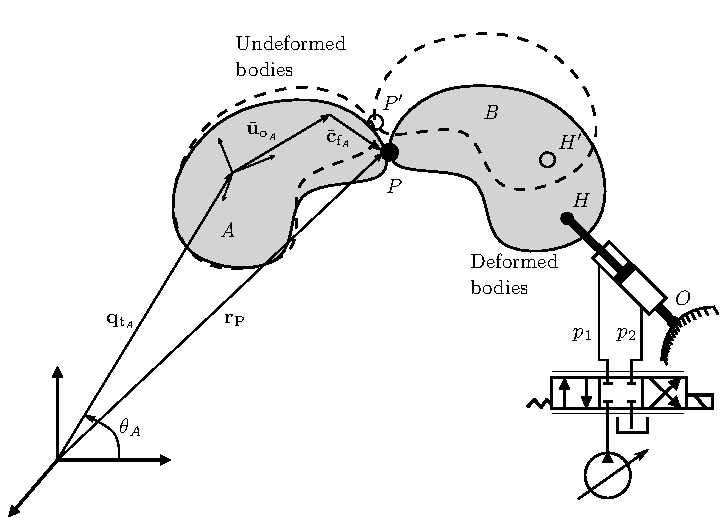
\includegraphics[width=\linewidth]{Fig1A.pdf}
        \caption{A hydraulically actuated flexible multibody system.}
        \label{Fig01A}
    \end{subfigure}
    \hfill
    \begin{subfigure}[b]{0.46\linewidth}
        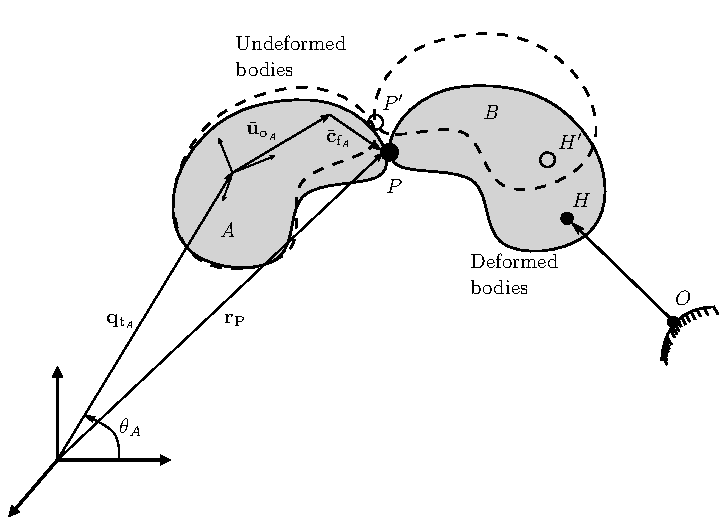
\includegraphics[width=\linewidth]{Fig1B.pdf}
        \caption{A surrogate-assisted flexible multibody system.}
        \label{Fig01B}
    \end{subfigure}
    \caption{\textbf{Coupled multibody systems}:~Coupling of flexible bodies with hydraulics and surrogates.}
    \label{Fig01}
\end{figure}
% The actuation system for these flexible bodies can be modeled using either: (a) a hydraulic system, or (b) a surrogate model.
%The hydraulic dynamics in such systems can also be replaced with the surrogate dynamics, see Fig.~\ref{fig01b}. This section further details 
\subsection{Flexible multibody system dynamics}
%\begin{figure}[h]
 %   \centering
  %  \begin{subfigure}[b]{0.45\linewidth}
   %    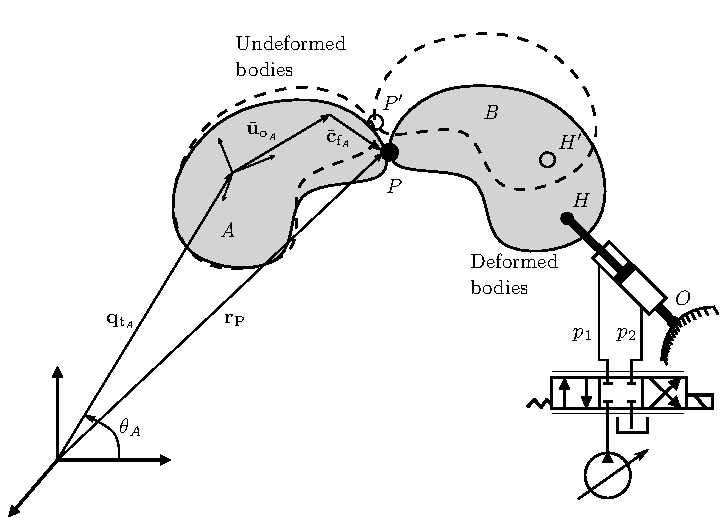
\includegraphics[width=\linewidth]{Fig1A.pdf}
        %\caption{Coupling of flexible multibody and hydraulic system dynamics.}
        %\label{fig:subfigA}
    %\end{subfigure}
    %\hfill
    %\begin{subfigure}[b]{0.45\linewidth}
     %   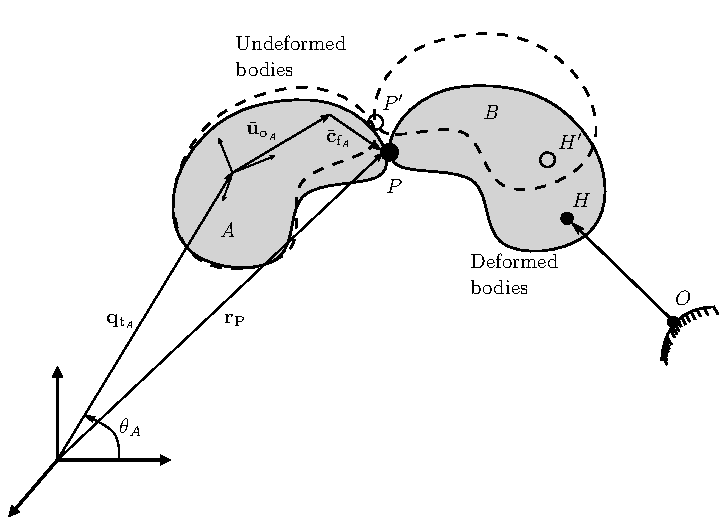
\includegraphics[width=\linewidth]{Fig1B.pdf}
      %  \caption{Coupling of flexible multibody and surrogate dynamics.}
       % \label{fig:subfigB}
    %\end{subfigure}
    %\caption{Flexible bodies \( A \) and \( B \) are connected at point \( P \), both in the undeformed and deformed states. The joint position can be described by the vector \(\mathbf{r}_p = \mathbf{q}_{t_A} + \mathbf{A}_{\boldsymbol{\theta}_A}(\bar{\mathbf{u}}_{o_A} + \bar{\mathbf{c}}_{f_A})\), where \( \mathbf{q}_{t_A} \in \mathbb{R}^{3 \times 1} \) represents the translational coordinate vector, \( \mathbf{A}_{\boldsymbol{\theta}_A} \) is the rotation matrix, and \( \boldsymbol{\theta}_A \in \mathbb{R}^{n_r \times 1} \) is the rotational parameterization vector, where \( n_r \) is the number of rotational degrees of freedom. The term \( \bar{\mathbf{u}}_{o_A} \) denotes the local coordinate vector, and \( \bar{\mathbf{c}}_{f_A} \in \mathbb{R}^{3 \times 1} \) represents the flexible coordinate vector. The actuation system for these flexible bodies can be modeled using either: (a) a hydraulic system, or (b) a surrogate model.}
    %\label{Fig01}
%\end{figure}

%A flexible body can deform under external forces and is assumed to be composed of an infinite number of particles~\cite{shabana2020dynamics}. These particles interact with each other. 
A flexible body can be defined with a generalized coordinate vector $\qv = {\begin{bmatrix}
\qv_{{\mathrm{t}}}^{\top} &
    {\Angle}^{\top} &
{\bar{\cv}}_{{\mathrm{f}}}^{\top} 
\end{bmatrix}}^{\top}$~\cite{shabana2020dynamics}, where \( \mathbf{q}_{t} \in \mathbb{R}^{3 \times 1} \), \( \boldsymbol{\theta} \in \mathbb{R}^{n_r \times 1} \) and  \( \bar{\mathbf{c}}_{f} \in \mathbb{R}^{3n_{\text{n}} \times 1} \) are the translational coordinate, rotational parameterization and flexible coordinate vectors, $n_r$ is the rotational degrees of freedom and $n_{\text{n}}$ is the number of nodes.~Fig.\ref{Fig01} demonstrates a system of two flexible bodies \( A \) and \( B \) connected at point \( P \), both in the undeformed and deformed states. 

Equations of motion for a coupled, constrained, flexible multibody system can be
demonstrated as~\cite{gerstmayr2023exudyn},
\begin{equation} \label{Eq01: GeneralEOM}
    {\Mm ({{\qv}})}{\ddot{\qv}} + { ({\Gv}_{{\qv}})^{\top} \lm}  = {{\Qv ({{\qv}}, {\dot{\qv}}, {{\uv}}, t)  }},
\end{equation}
\begin{equation} \label{Eq01: GeneralEOM1}
    {{\Gv} ({{\qv}},t)} = {\mathbf{0}}, \quad~\text{and}
\end{equation}
\begin{equation} \label{Eq03: GeneralEOM1}
 \dot{\ODEy} + \frac{\partial \Gv}{{\partial {\ODEy} }^{\top}} \lm = {{\mathbf{f}_{\ODE}} ({{\qv}}, {\dot{\qv}}, {{\uv}}, t)}, 
\end{equation}
where ${{\qv}}$, ${\dot{\qv}}$ and  ${\ddot{\qv}} \in \Rcal^{n}$ are the generalized position, velocity and acceleration vectors, ${\Mm} \in \Rcal^{n \times n }$ is the system mass matrix, ${\Gv}_{{\qv}}$ is the jacobian of {holonomic} constraint equations ${{\Gv}}$, $\lm$ is the vector of Lagrange-multipliers, ${\Qv \in \Rcal^{n}}$ is generalized force vector, ${{\uv}}$ is the control signal  and $n$ is the number of coordinates in the system.
%The dynamics of such systems can be described in differential form using the classical formulations in the multibody system dynamics  as~\cite{gerstmayr2023exudyn,khadim2025real},
%\begin{equation} \label{Eq01: GeneralEOM}
 %   {\Mm ({{\qv}})}{\ddot{\qv}} + { ({\Gv}_{{\qv}})^{\top} \lm}  = {{\Qv ({{\qv}}, {\dot{\qv}}, {{\uv}}, t)  }},
%\end{equation}
%\begin{equation} \label{Eq01: GeneralEOM1}
 %   {{\Gv} ({{\qv}},t)} = {\mathbf{0}}, \quad~\text{and}
%\end{equation}
%\begin{equation} \label{Eq03: GeneralEOM1}
 %\dot{\ODEy} + \frac{\partial \Gv}{{\partial {\ODEy} }^{\top}} \lm = {{\mathbf{f}_{\ODE}} ({{\qv}}, {\dot{\qv}}, {{\uv}}, t)}, 
%\end{equation}
%where ${{\qv}}$, ${\dot{\qv}}$, and ${\ddot{\qv}}$ are the generalized position, velocity, and acceleration vectors, ${\Mm}$ is the system mass matrix, ${\Gv}_{{\qv}}$ is the Jacobian of the holonomic constraint equations ${{\Gv}}$, $\lm$ is the vector of Lagrange multipliers, ${\Qv}$ is the generalized force vector, ${{\mathbf{f}_{\ODE}}}$ is the first-order ordinary differential equations of a variable $\mathbf{y}$ and ${{\uv}}$ is the control input vector. In case of hydraulics, $\dot{\ODEy}$ in Eq.~\eqref{Eq03: GeneralEOM1} is replaced by the pressure equations~\cite{khadim2025real}.

Using the modal coordinates ${{\mathbf{\zeta}}} \in \Rcal^{3n_{\text{m}} \times 1}$, $\bar{\mathbf{c}}_{f}$ can be reduced as ${\bar{\cv}}_{{\mathrm{f}}} \approx {\overline{\NNPara}} {{\mathbf{\zeta}}},~\text{with}~n_{\text{m}}=\dim({{\mathbf{\zeta}}}) \ll \dim({\bar{\cv}}_{{\mathrm{f}}}) = 3n_{\text{n}}$ in CMS, where $n_{\text{m}}$ is the modal coordinates, and ${\overline{\NNPara}}_\text{A}  \in \Rcal^{3n_{\text{n}} \times n_{\text{m}}}$ is the column-wise modes reduction-basis~\cite{zwlfer_2019_a,zwolfer2021nodal}. For a flexible multibody system, the definition of joint and constraint equations is further detailed using the modally reduced CMS in~\cite{Johannes2024}.

For a flexible multibody system, ${\Mm}$ and ${\Qv}$ can be defined using the modally reduced Component Mode Synthesis (CMS)~\cite{zwolfer2021nodal} as,
\begin{equation} \label{Eq03_04: ConstraintsAndForces1}
{\Mm} = {\begin{bmatrix}
    {{\mathbf{\widehat{M}_{\text{tt}}}}}  & {{\mathbf{\widehat{M}_{\text{tr}}}}} & {{\mathbf{\widehat{M}_{\text{tf}}}}}\\
    & {{\mathbf{\widehat{M}_{\text{rr}}}}} & {{\mathbf{\widehat{M}_{\text{rf}}}}} \\
    \text{sym.} &  & {{\mathbf{\widehat{M}_{\text{ff}}}}}
\end{bmatrix}},  
\end{equation}
\begin{equation} \label{Eq03_04: ConstraintsAndForces2}
{ ({\Gv}_{{\qv}})^{\top} \lm} = \underbrace{\begin{bmatrix}
     \mathbf{\widehat{Q}_{\text{c}_{\text{t}}}} \\
     \mathbf{\widehat{Q}_{\text{c}_{\text{r}}}} \\
     \mathbf{\widehat{Q}_{\text{c}_{\text{f}}}} 
\end{bmatrix}}_{\substack{\text{constraint force} \\ \text{vector}}}, \quad~\text{and}
\end{equation}
\begin{equation} \label{Eq03_04: ConstraintsAndForces}
\Qv = \underbrace{\begin{bmatrix}
     \mathbf{\widehat{Q}_{\text{e}_{\text{t}}}} \\
     \mathbf{\widehat{Q}_{\text{e}_{\text{r}}}} \\
     \mathbf{\widehat{Q}_{\text{e}_{\text{f}}}} 
\end{bmatrix}}_{\substack{\text{elastic force} \\ \text{vector}}} + \underbrace{\begin{bmatrix}
     \mathbf{\widehat{Q}_{\text{v}_{\text{t}}}} \\
     \mathbf{\widehat{Q}_{\text{v}_{\text{r}}}} \\
     \mathbf{\widehat{Q}_{\text{v}_{\text{f}}}} 
\end{bmatrix}}_{\substack{\text{quadratic velocity} \\ \text{vector}}}+ \underbrace{\begin{bmatrix}
     \mathbf{\widehat{Q}_{\text{a}_{\text{t}}}} \\
     \mathbf{\widehat{Q}_{\text{a}_{\text{r}}}} \\
     \mathbf{\widehat{Q}_{\text{a}_{\text{f}}}} 
\end{bmatrix}}_{\substack{\text{applied force} \\ \text{vector}}}.
\end{equation}
Further details of terms in $\Mm$ and $\Qv$ can be found can be found in~\cite{zwolfer2021nodal}. 
%Further details about ${{\mathbf{\widehat{M}_{\text{tt}}}}}$, ${{\mathbf{\widehat{M}_{\text{tr}}}}}$,  ${{\mathbf{\widehat{M}_{\text{tf}}}}}$, ${{\mathbf{\widehat{M}_{\text{rr}}}}}$, ${{\mathbf{\widehat{M}_{\text{rf}}}}}$, ${{\mathbf{\widehat{M}_{\text{ff}}}}}$, $\mathbf{\widehat{Q}_{\text{c}_{\text{t}}}}$,$\mathbf{\widehat{Q}_{\text{c}_{\text{r}}}}$,$\mathbf{\widehat{Q}_{\text{c}_{\text{f}}}}$,   $\mathbf{\widehat{Q}_{\text{e}_{\text{t}}}}$,$\mathbf{\widehat{Q}_{\text{e}_{\text{r}}}}$, $\mathbf{\widehat{Q}_{\text{e}_{\text{f}}}}$,  $\mathbf{\widehat{Q}_{\text{v}_{\text{t}}}}$,$\mathbf{\widehat{Q}_{\text{v}_{\text{r}}}}$,$\mathbf{\widehat{Q}_{\text{v}_{\text{f}}}}$,  $\mathbf{\widehat{Q}_{\text{a}_{\text{t}}}}$,$\mathbf{\widehat{Q}_{\text{a}_{\text{r}}}}$ and $\mathbf{\widehat{Q}_{\text{a}_{\text{f}}}}$ in Eqs.~\eqref{Eq03_04: ConstraintsAndForces1}--\eqref{Eq03_04: ConstraintsAndForces} can be found in~\cite{zwolfer2021nodal}. In a flexible multibody system, the definition of joint and constraint equations is further detailed in~\cite{Johannes2024} using the modally reduced CMS.

\subsection{Coupling with hydraulics}
The dynamics of a flexible body and hydraulics can be coupled using the Lumped Fluid theory~(LFT) \cite{khadim2025real,watton2009fundamentals}. Fig.~\ref{Fig01A} demonstrates a hydraulic actuator between the nodes $H$ and $O$. A hydraulic actuator is connected to the flexible body $B$ through a standard RBE2-interface at $H$~\cite{khadim2025real}. 

The position vector $\mathbf{r}_{OH}$ couples the hydraulic force $F_h$ produced by actuator with the flexible body. The hydraulic force can be described in vector form as, 
${\mathbf{F}_h} =F_h \mathbf{r}_{OH}$. The force ${F}_{h}$ can be described as,
\begin{equation} \label{Hydraulicforce}
{F}_{h}  =  p_{h_1}A_{h_1} - p_{h_2}A_{h_2} -F_{\mu},
\end{equation}
where $p_{h_1}$ and $p_{h_2}$ are the pressures, $A_{h_1}$ and $A_{h_2}$ are the cylinder areas and $F_{\mu}$ is the cylinder friction force. The force $F_{\mu}$ in the hydraulic cylinder is computed according to~\cite{brown2016continuous}. The hydraulic pressure~$p_{h_i}$ can be expressed through a hydraulic volume ${V_{h_i}}$ as,
\begin{equation} \label{DiffPressure}
\dot{p}_{h_i}  = \frac{B_{e_{h_i}}}{V_{h_i}}  \left(- \frac{d {V_{h_i}}}{dt} + Q_{s_i}  \right), 
\end{equation}
\begin{equation} \label{EffectBulk}
    B_{e_{h}} = \left(\frac{1}{B_{o}} + \sum_{c=1}^{n_{h}} \frac{V_{c}}{{V_{h}}{B_{c}}} \right)^{-1}
\end{equation}
where $B_{e_{h_i}}$ is the effective bulk modulus, $Q_{s_i}$ is the flow rate, $B_{\mathrm{o}}$ is the oil bulk modulus, $B_{\mathrm{c}}$ is the bulk modulus in a sub-volume  $V_{\mathrm{c}}$ and ${n_{h}}$ is the total number of hydraulic volumes. For a hydraulic system, $\dot{\mathbf{y}}$ in Eq.~\eqref{Eq03: GeneralEOM1} is replaced by the hydraulic pressure derivative, $\dot{p}_{h_i}$. At an arbitrary $i^{th}$ node, ${{\mathbf{F}}_{\mathrm{h}}}$ is described into a nodal force vector ${{\mathbf{f}}_{\mathrm{a}}}^{(i)}$ as, 
\begin{equation}\label{Eq04: NodalHydraulicForce}
    {{\mathbf{f}}_{\mathrm{a}}}^{(i)} = {w^{(i)}} {{\mathbf{F}}_{\mathrm{h}}},
\end{equation}
where ${w^{(i)}} = \frac{1}{3A_B} \sum_{\text{j}} A_{\text{j}}, \quad \sum_i {w^{(i)}} = 1$ is the nodal weighting, $A_{\text{j}}$ is the area of each triangle ${\text{j}}$ and $A_B$ is the total boundary area. The weighting factor ensures nearly constant strain distribution with equally distributed axial hydraulic forces. In a monolithic coupling, Eq.~\eqref{Eq03_04: ConstraintsAndForces} can be expressed into form  
${{\mathbf{f}}_{\mathrm{a}}}^{(i)}$  as, 
%a position vector~\cite{khadim2025real}. 
\begin{equation}\label{Eq03: AppliedForce1}
 {{\mathbf{\widehat{Q}_{\text{a}_{\text{t}}}}}} = \displaystyle\sum_{i=1}^{{n_{\text{n}}}} {{\mathbf{f}}_{\mathrm{a}}}^{(i)}, \quad {{\mathbf{f}}_{\mathrm{a}}}^{(i)} \neq 0, 
\end{equation}
\begin{equation}\label{Eq03: AppliedForce2}
{{\mathbf{\widehat{Q}_{\text{a}_{\text{r}}}}}} = {\overline {\Gv}}^{\top} \displaystyle\sum_{i=1}^{{n_{\text{n}}}}
\begin{bmatrix}
{\widetilde{\overline{\ix}}}^{(i)} + \displaystyle\sum_{\text{m}=1}^{{n_{\text{m}}}}{\widetilde{\overline{\NNPara}}_{\text{m}}}^{(i)} \mathbf{\zeta}_\text{m} \end{bmatrix}
\mathbf{A}^{\top} {{\mathbf{f}}_{\mathrm{a}}}^{(i)}, \quad {{\mathbf{f}}_{\mathrm{a}}}^{(i)} \neq 0, \quad~\text{and}
\end{equation}
\begin{equation}\label{Eq03: AppliedForce3}
{{\mathbf{\widehat{Q}_{\text{a}_{\text{f}}}}}} = \displaystyle\sum_{i=1}^{{n_{\text{n}}}} 
\left[ 
\begin{array}{c}
\overline{\NNPara}_1^{(i)^{\top}} \\
\vdots \\
\overline{\NNPara}_{{n_{\text{m}}}}^{(i)^{\top}}
\end{array}
\right] 
\mathbf{A}^{\top} {{\mathbf{f}}_{\mathrm{a}}}^{(i)}, \quad {{\mathbf{f}}_{\mathrm{a}}}^{(i)} \neq 0, 
\end{equation}
where $\mathbf{A}$ is the transformation matrix and ${{\widetilde{\overline{\ix}}}^{(i)}}$ is the undeformed (reference) nodal
coordinates.


%The first-order-differential Eq.~\eqref{Eq03: GeneralEOM1} demonstrates hydraulic actuator, thermal or electric dynamics in a coupled mechanical system~\cite{ikaheimo2024real,khadim2025real}. 

%\subsection{Simulation-driven approach}
\begin{figure}[ht]
    \centering
    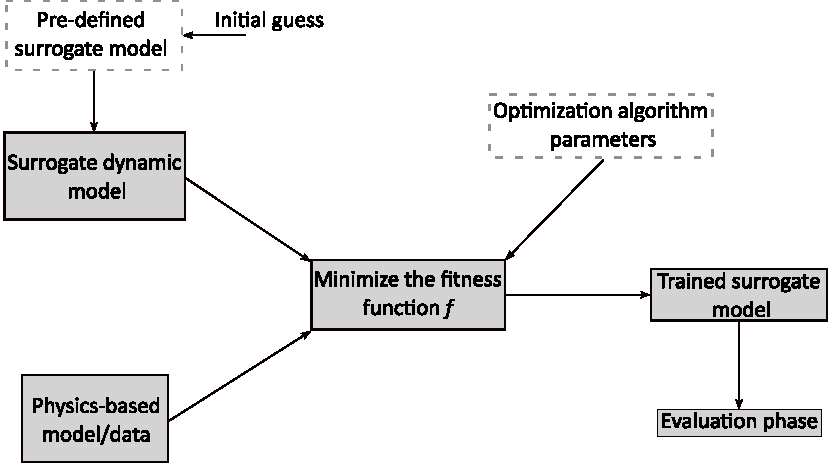
\includegraphics[width=0.9\linewidth]{Fig02.pdf}
    \caption{Pre-defined surrogate model-based training workflow to identify hydraulic parameters. }
    \label{fig:optimization}
\end{figure}
\subsection{Surrogate dynamics}
As shown in Fig.~\ref{Fig01B}, the surrogate solution replaces hydraulics for a coupled multibody system~\cite{khadim2024simulation}.~These solutions are obtained in a training process shown in Fig.~\ref{fig:optimization}. This workflow utilizes a predefined surrogate model compared to conventional data-driven surrogates~\cite{han2024data,manzl2024slide,khadim2025real}. 

The objective of training is to minimize the fitness function ${f}$. It can be defined as the Mean Square Error (MSE),
\begin{equation}
 \label{FitnessFunction}
     f = \frac{1}{{\nTrain}} \sum_{i=1}^{\nTrain} ({\widehat{\InputLayer}}_{i} - \InputLayer)^2
\end{equation}
where $\nTrain$ is the number of training steps,~${\widehat{\InputLayer}}_{i}$ is the input vector from surrogate dynamic model and ${{\InputLayer}}$ is the input vector from the physics-based model.~The proposed workflow uses CMA-ES optimization algorithm~\cite{hansen2003reducing} to minimize $f$. The surrogate dynamic model is function of pre-defined surrogate force model ${F}_{s}$~\cite{khadim2024simulation}, 
\begin{equation} \label{Surrogate}
{F}_{s}  =  aU + b_0 + b_1s_0 + b_2{\mathbf{s}} + b_3\dot{{\mathbf{s}}},
\end{equation}
where $s_0$ initial actuator length, ${\mathbf{s}}$ is the actuator position, $\dot{{\mathbf{s}}}$ is the actuator velocity, $a$, $b_0$, $b_1$, $b_2$ and $b_3$ are the initial guess of surrogate force parameters. 

After training process, the optimal surrogate force parameters are determined to calculate~$F_s$, which can replace an equivalent force $F_h$. Thus, $\dot{\ODEy}$ is not required in computing Eqs.~\eqref{Eq01: GeneralEOM}--\eqref{Eq03: GeneralEOM1} for solving coupled flexible multibody system dynamics. In~\cite{khadim2024simulation}, ${\mathbf{s}}$ and $\dot{{\mathbf{s}}}$ were used to compute the fitness function~$f$. It can be expressed as, 
\begin{equation}
    f = f_1+f_2
\end{equation}
where $f_1$ and $f_2$ are computed according to Eq.~\eqref{FitnessFunction}.
\section{Case example: Flexible forestry crane}

A forestry crane, commonly used in the forest industry for handling logs and heavy materials, serves as the case example in this study. Its mechanical subsystem comprises a pillar, lift boom, tilt boom, and two brackets (Bracket One and Bracket Two), as shown in Figure \ref{fig01a} and detailed in Figure \ref{fig01b}. 
% The components’ mass, inertial, and geometric properties are listed in Table \ref{Tab01}.


\begin{figure}[h]
    \begin{subfigure}{0.5\textwidth} 
        \centering
        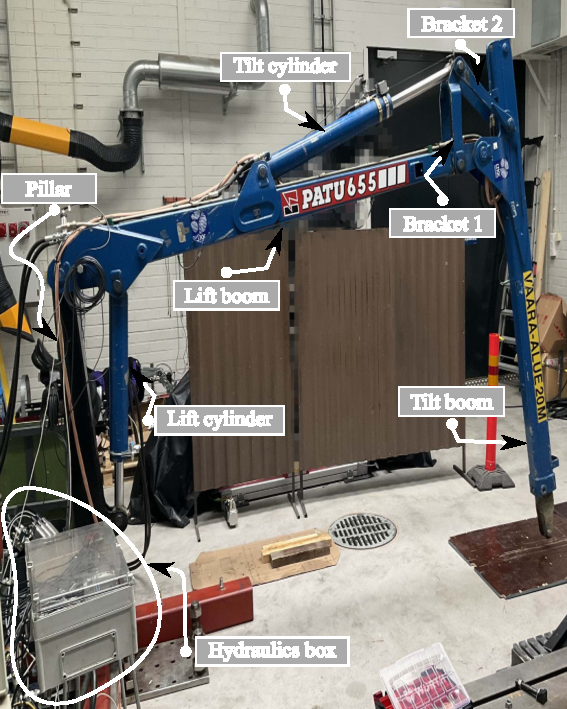
\includegraphics[width=1.82in]{Fig2A.pdf}
        \caption{}
        \label{fig01a}
    \end{subfigure}%
    \hfill
    \begin{subfigure}{0.5\textwidth} 
        \centering
        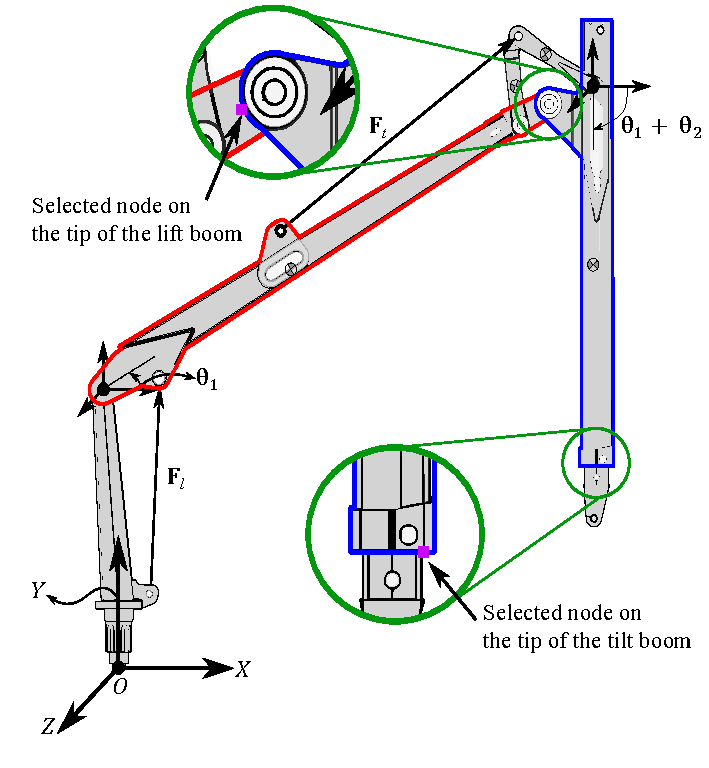
\includegraphics[width=1.82in]{Fig2B.pdf}
        \caption{}
        \label{fig01b}
    \end{subfigure}
    \caption{Example of a forestry crane: (a) Experimental setup at the Laboratory of Intelligent Machines, LUT University, and (b) The lift boom (outlined in red) and the tilt boom (outlined in blue) were modeled as flexible body components in this study. Two nodes at the tip of each boom were selected to investigate the deflection of these flexible parts.}
    \label{Fig:SurrogateForestry}
\end{figure}


% \begin{table}[h]
% \caption{The mass, inertial, and geometric properties of the mechanical building blocks of the forestry crane.}
% \label{Tab01}
% \centering
% \begin{tabular}{lccccccc} % Updated column count to 8
% \hline
% Body & Mass (kg) & Inertia & Length(m) & Height(m) & x(m) & y(m) \\
% \hline
% Pillar & 88.207 & 1.675 & 0.344 & 1.426 & -0.017 & 0.578 \\
% Lift boom & 123.764 & 3.700 & 2.959 & 0.392 & 1.120 & 0.030 \\
% Bracket 1 & 11.524 & 0.266 & 0.131 & 0.545 &  0.004 & 0.257 \\
% Bracket 2 & 7.900 & 0.207 & 0.575 &  0.1  & 0.213 & 0 \\
% Tilt Boom & 76.213 &  2.735 & 2.270 & 0.417 & 0.498 & 0.239 \\
% \hline
% \end{tabular}
% \end{table}


\subsection{Flexible multibody model}
    
% The multibody model of the forestry crane comprises five interconnected bodies: the pillar, lift boom, and tilt boom are linked sequentially, while Bracket One and Bracket Two form a closed loop between the lift and tilt booms. All connections use revolute joints, except for Brackets One and Two, which are joined by a spherical joint. A cut joint between the brackets removes redundancy and ensures numerical stability during simulation.

% The default building blocks of the mechanical system in this study were rigid components. However, the lift boom and tilt boom were modeled as flexible bodies, as they experience the most deformation and are thus the critical components in terms of flexibility. To account for this, modal analysis was performed on the 3D CAD models of these two parts using ANSYS Workbench 2022 R2. Ten-node tetrahedral elements (Tet10) were used as the default elements for meshing. The mesh statistics included 41,873 nodes and 21,734 elements for the lift boom and 74,759 nodes and 38,994 elements for the tilt boom. To generate the flexible parts, the modal analysis results were exported to Exudyn as the simulation environment. The detailed description for the rest of the mechanical subsystems can be found in the study by Khadim et al.~\cite{KHADIM2023105405}.
    
% Modal reduction was applied to the analysis results before generating flexible bodies to reduce problem size and computational load. In this study, the Craig-Bampton method was used for this purpose. While including more modes improves simulation accuracy, it also increases computational complexity. To balance accuracy and efficiency, rigid modes were excluded, and representative normal, bending, and torsional modes were selected within the 100–450 Hz range to capture different deformation conditions. The chosen modes were 118.37 Hz, 155.4 Hz, and 314.77 Hz for the lift boom, and 145.79 Hz, 208.67 Hz, and 403.12 Hz for the tilt boom.
The multibody model of the forestry crane includes five interconnected bodies: the pillar, lift boom, and tilt boom are sequentially linked, while Brackets One and Two form a closed loop between the lift and tilt booms. 
\begin{figure}[ht]
    \begin{subfigure}{0.5\textwidth} 
        \centering
        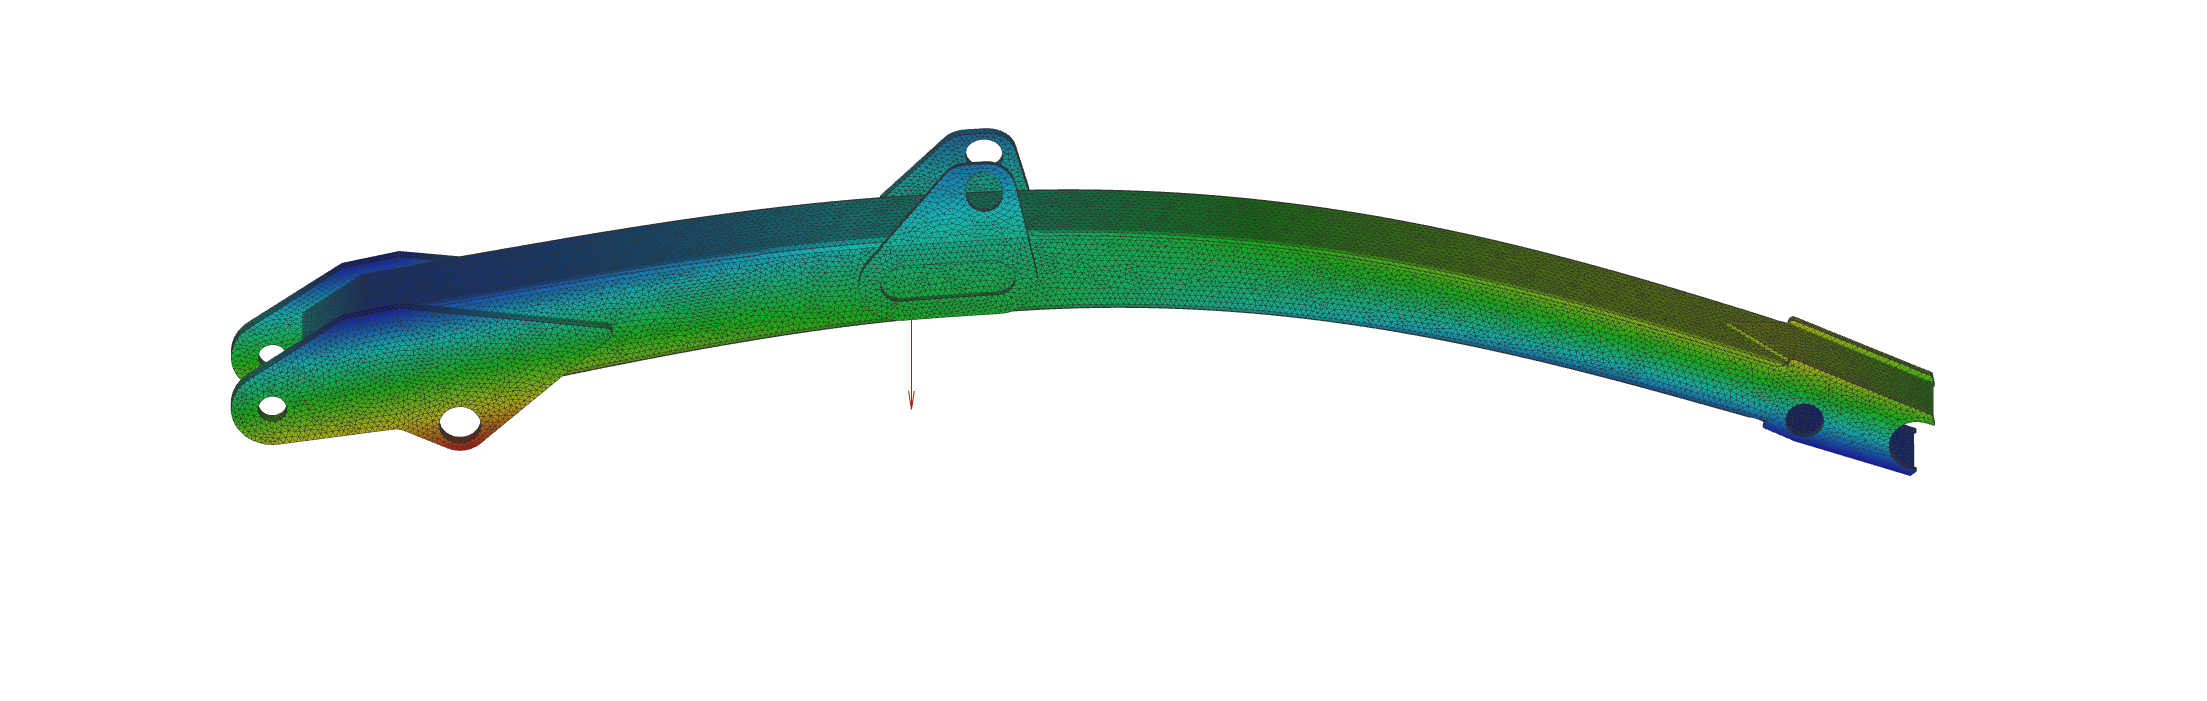
\includegraphics[width=1.82in]{LB01.png}
        \caption{103.96 Hz}
        \label{LiftSurrogate}
    \end{subfigure}%
    \begin{subfigure}{0.5\textwidth} 
        \centering
        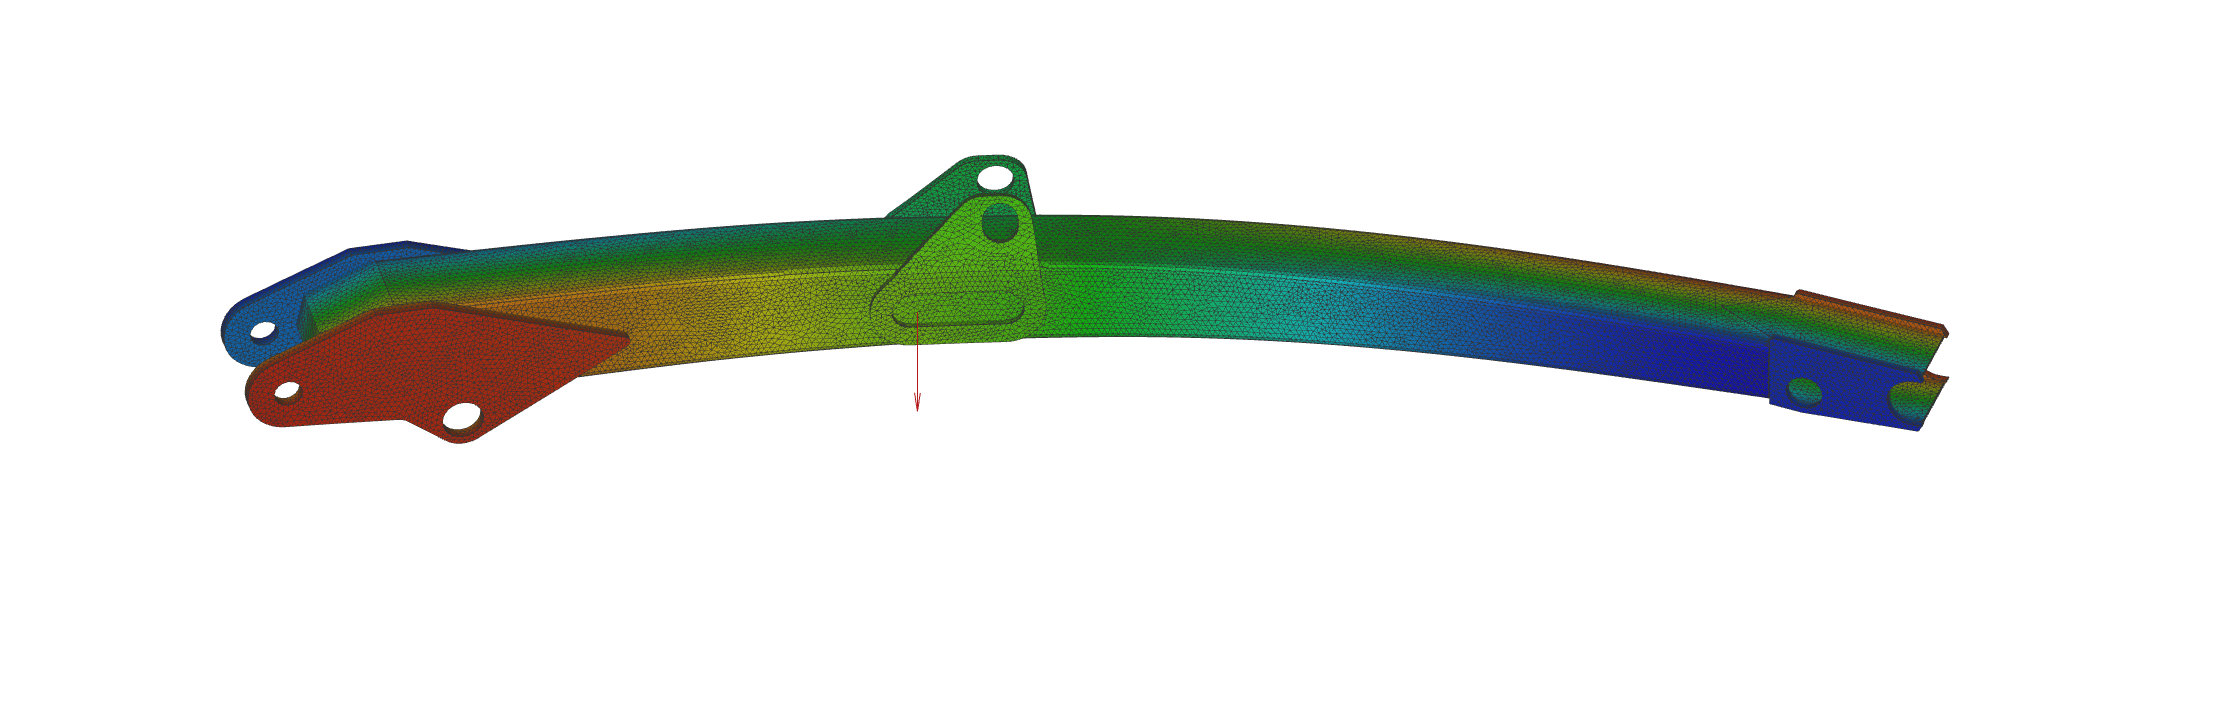
\includegraphics[width=1.82in]{LB02.png}
        \caption{110.11 Hz}
        \label{TiltSurrogate}
    \end{subfigure}
    \begin{subfigure}{0.5\textwidth} 
        \centering
        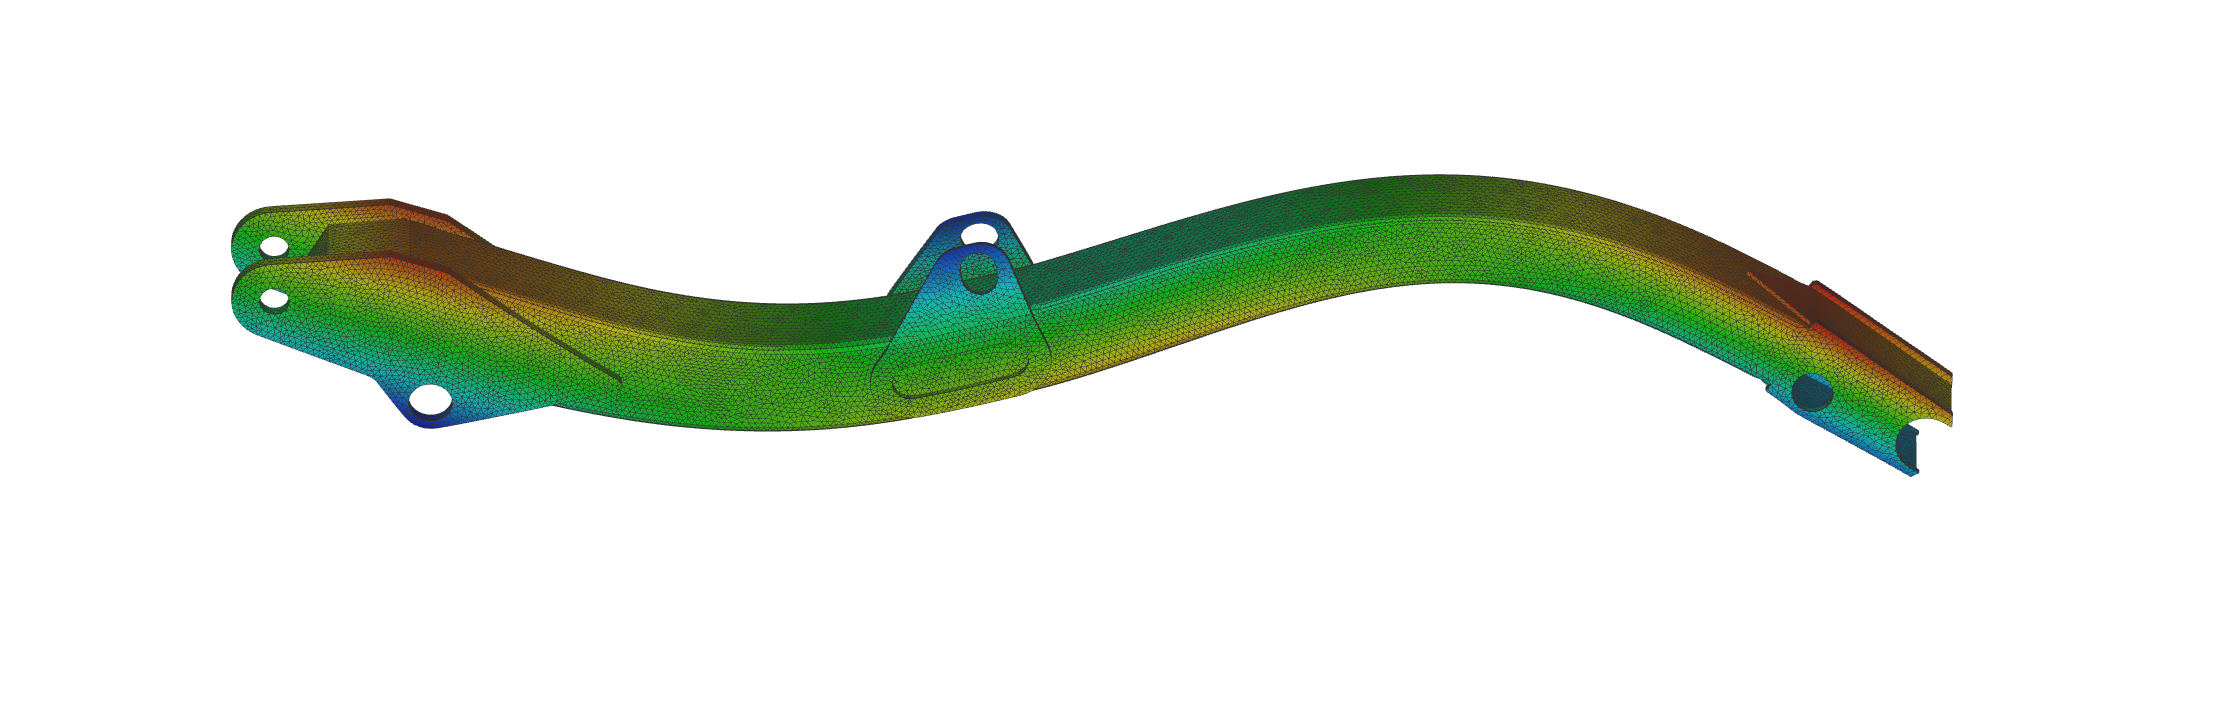
\includegraphics[width=1.82in]{LB03.png}
        \caption{296.70 Hz}
        \label{LiftSurrogate}
    \end{subfigure}%
    \begin{subfigure}{0.5\textwidth} 
        \centering
        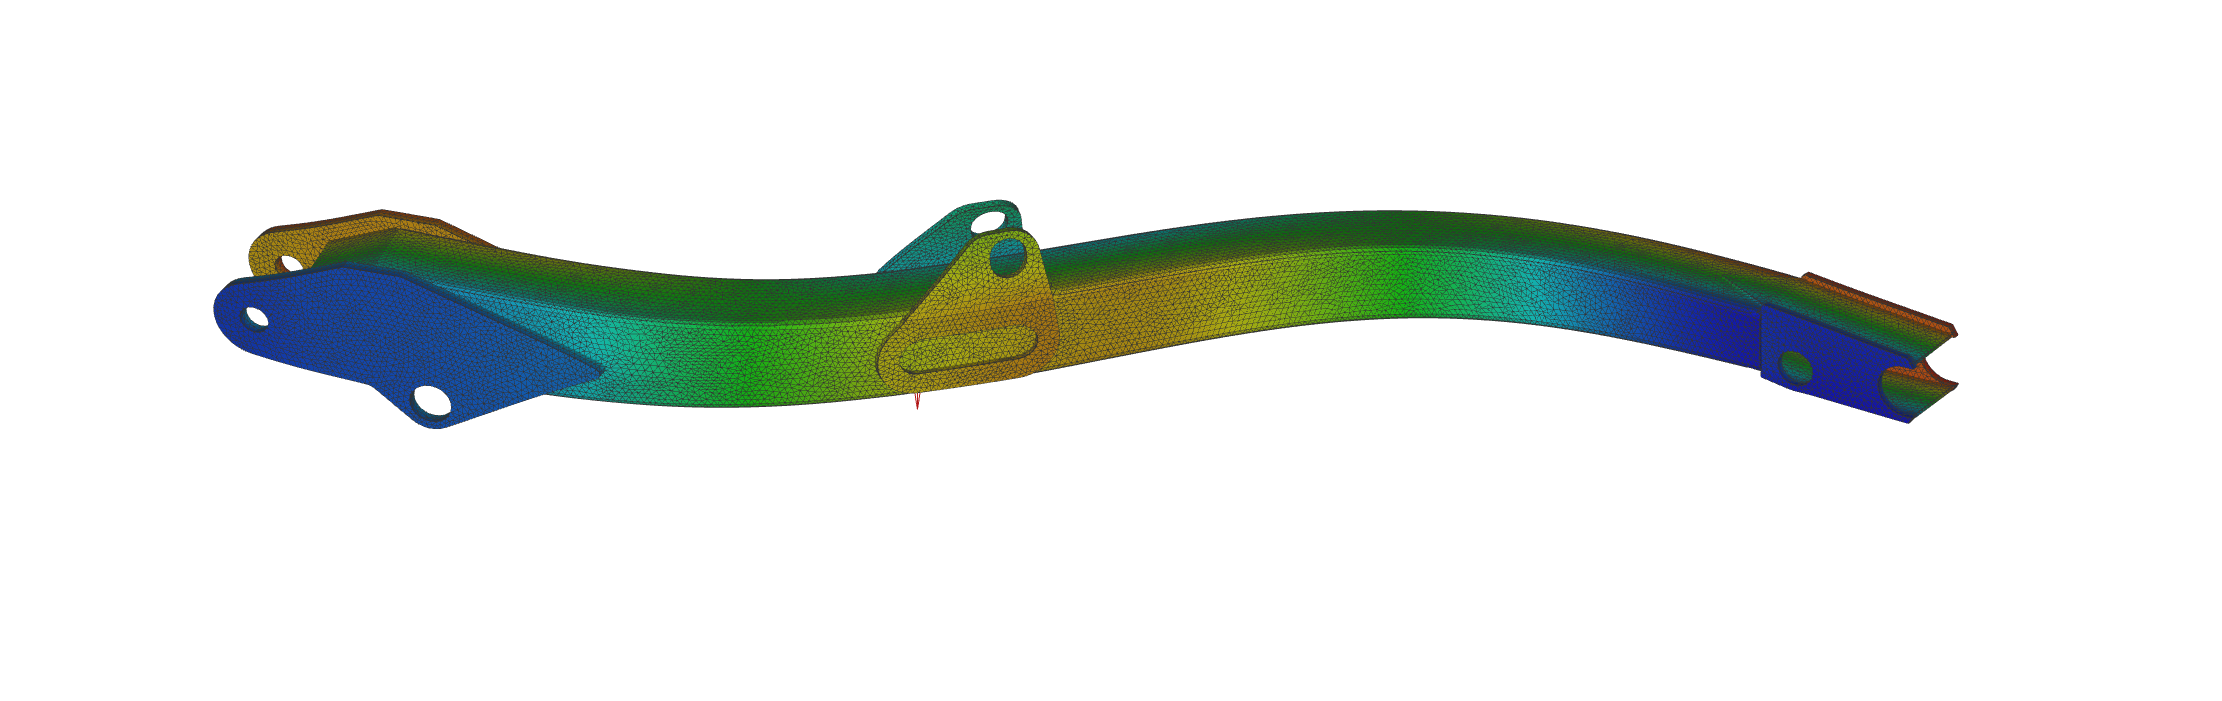
\includegraphics[width=1.82in]{LB04.png}
        \caption{309.68 Hz}
        \label{TiltSurrogate}
    \end{subfigure}
    \begin{subfigure}{0.5\textwidth} 
        \centering
        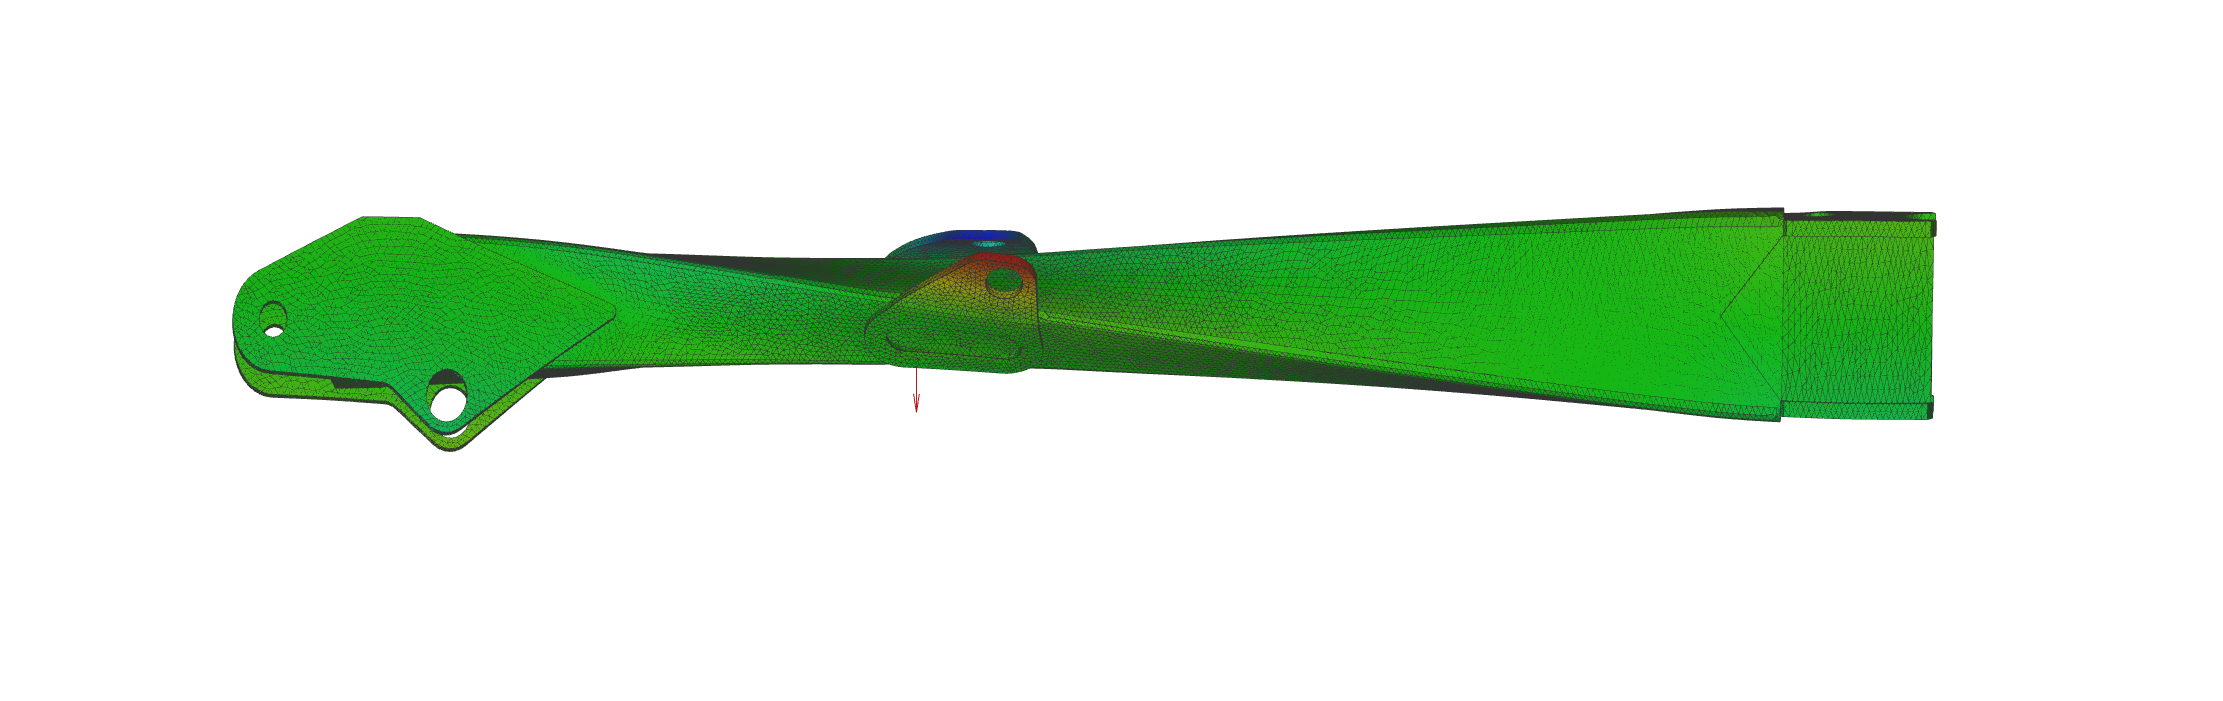
\includegraphics[width=1.82in]{LB05.png}
        \caption{399.19 Hz}
        \label{LiftSurrogate}
    \end{subfigure}%
    \begin{subfigure}{0.5\textwidth} 
        \centering
        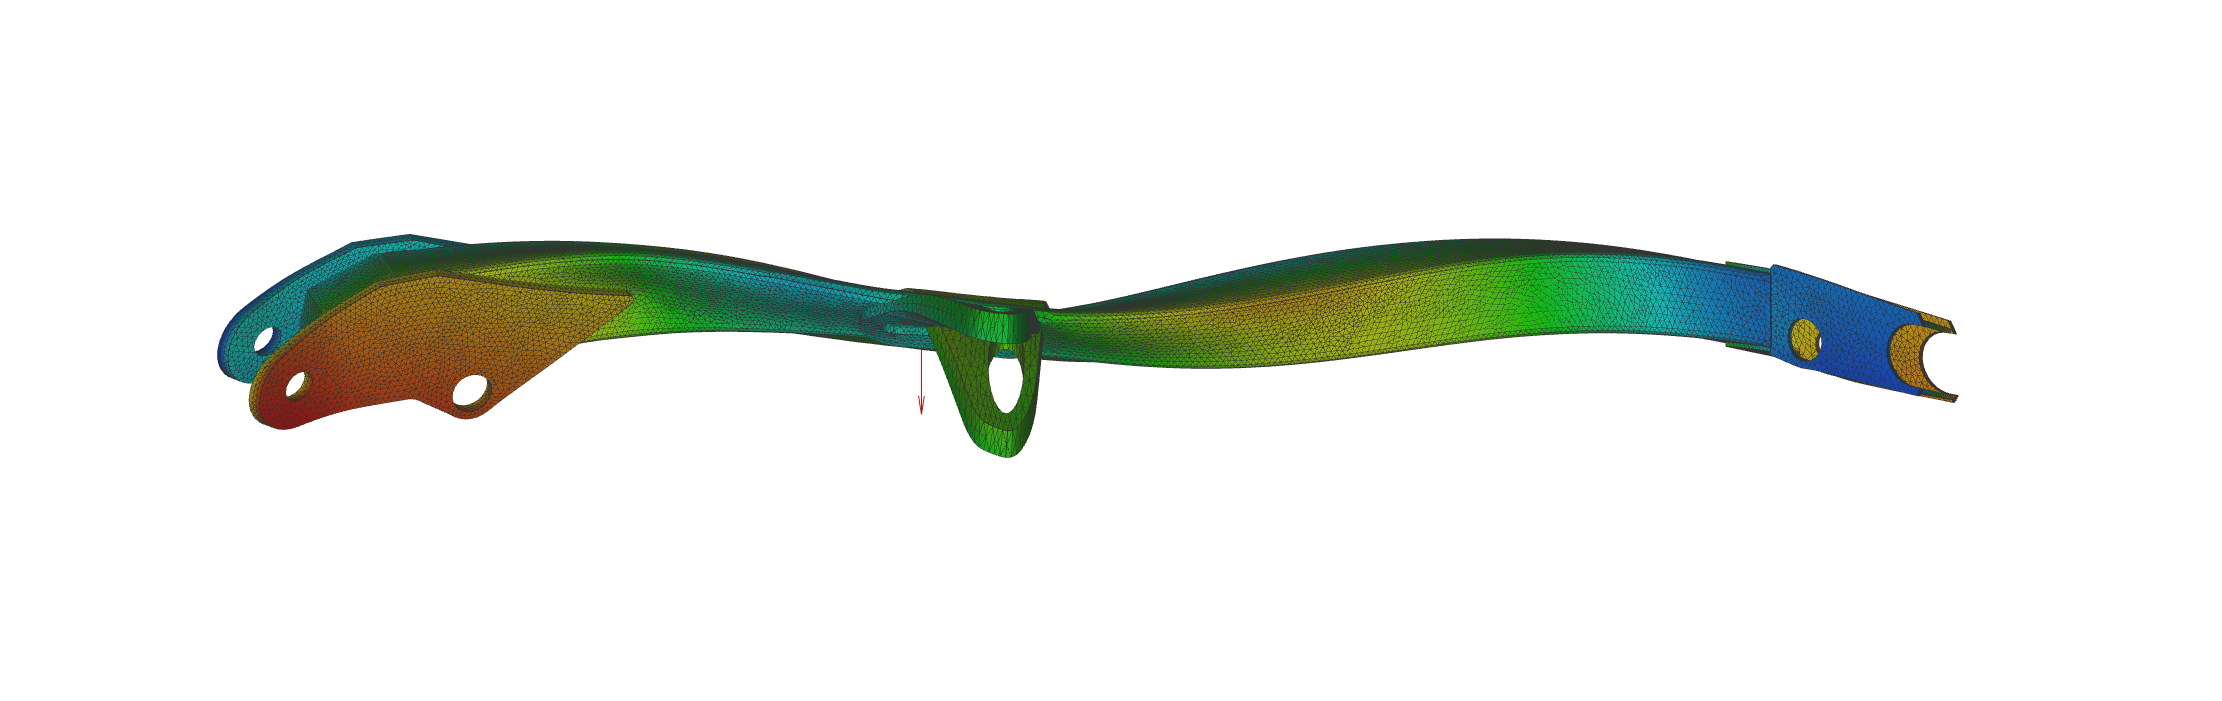
\includegraphics[width=1.82in]{LB06.png}
        \caption{524.90 Hz}
        \label{TiltSurrogate}
    \end{subfigure}
        \begin{subfigure}{0.5\textwidth} 
        \centering
        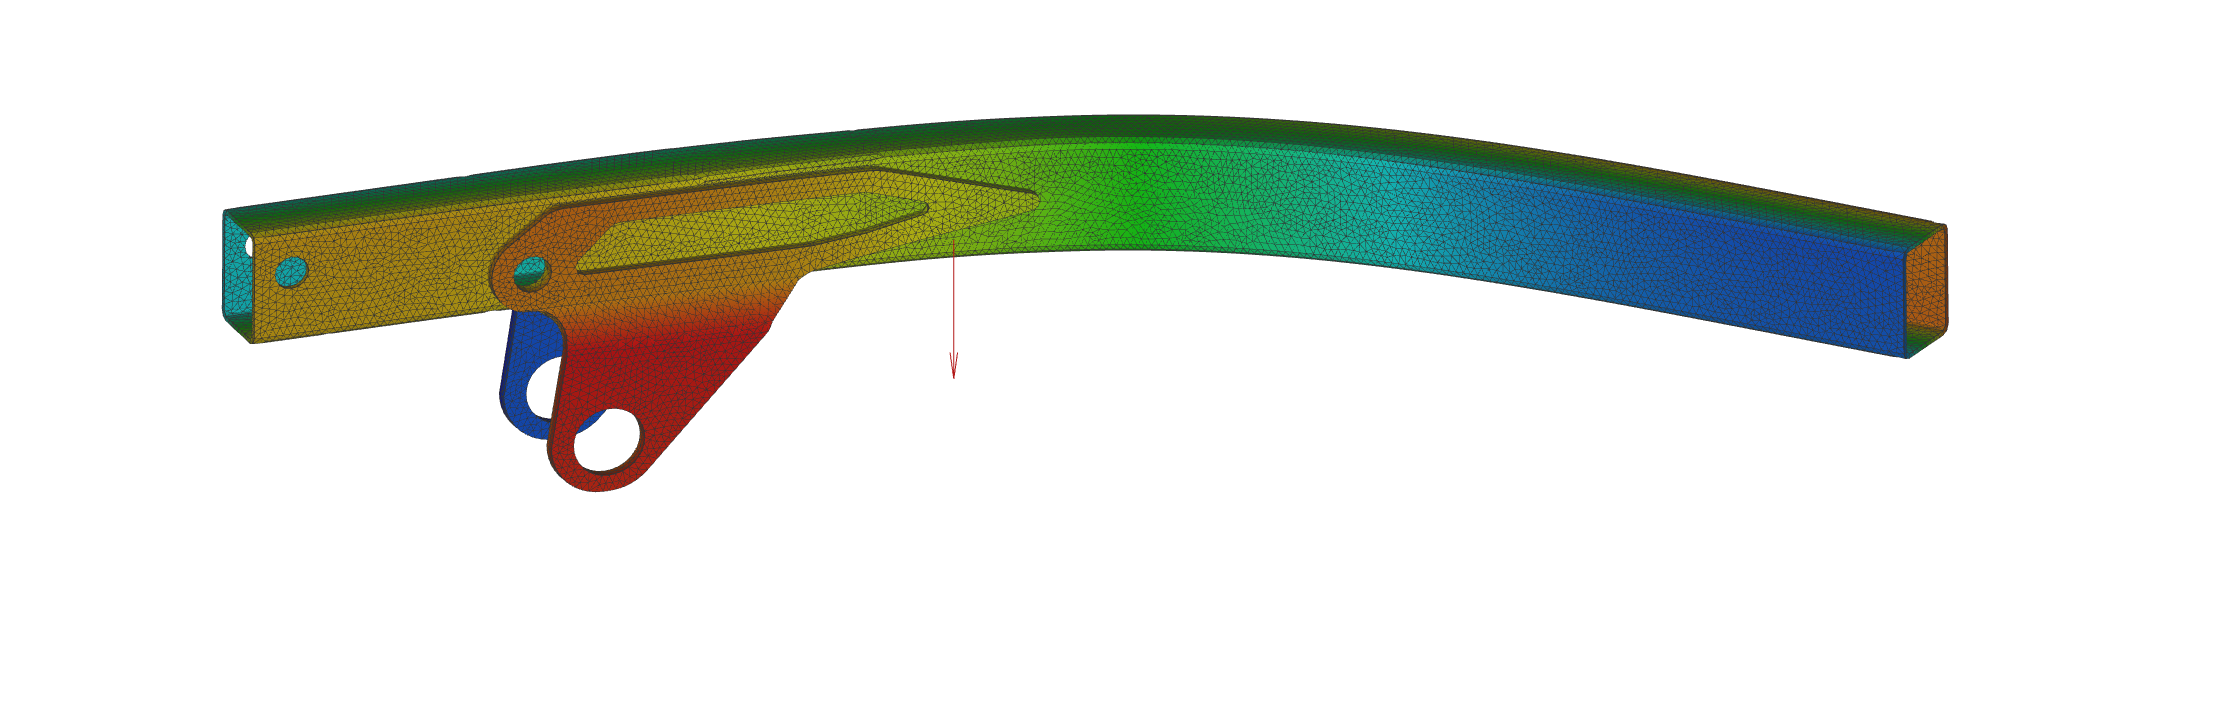
\includegraphics[width=1.82in]{TB01.png}
        \caption{149.76 Hz}
        \label{LiftSurrogate}
    \end{subfigure}%
    \begin{subfigure}{0.5\textwidth} 
        \centering
        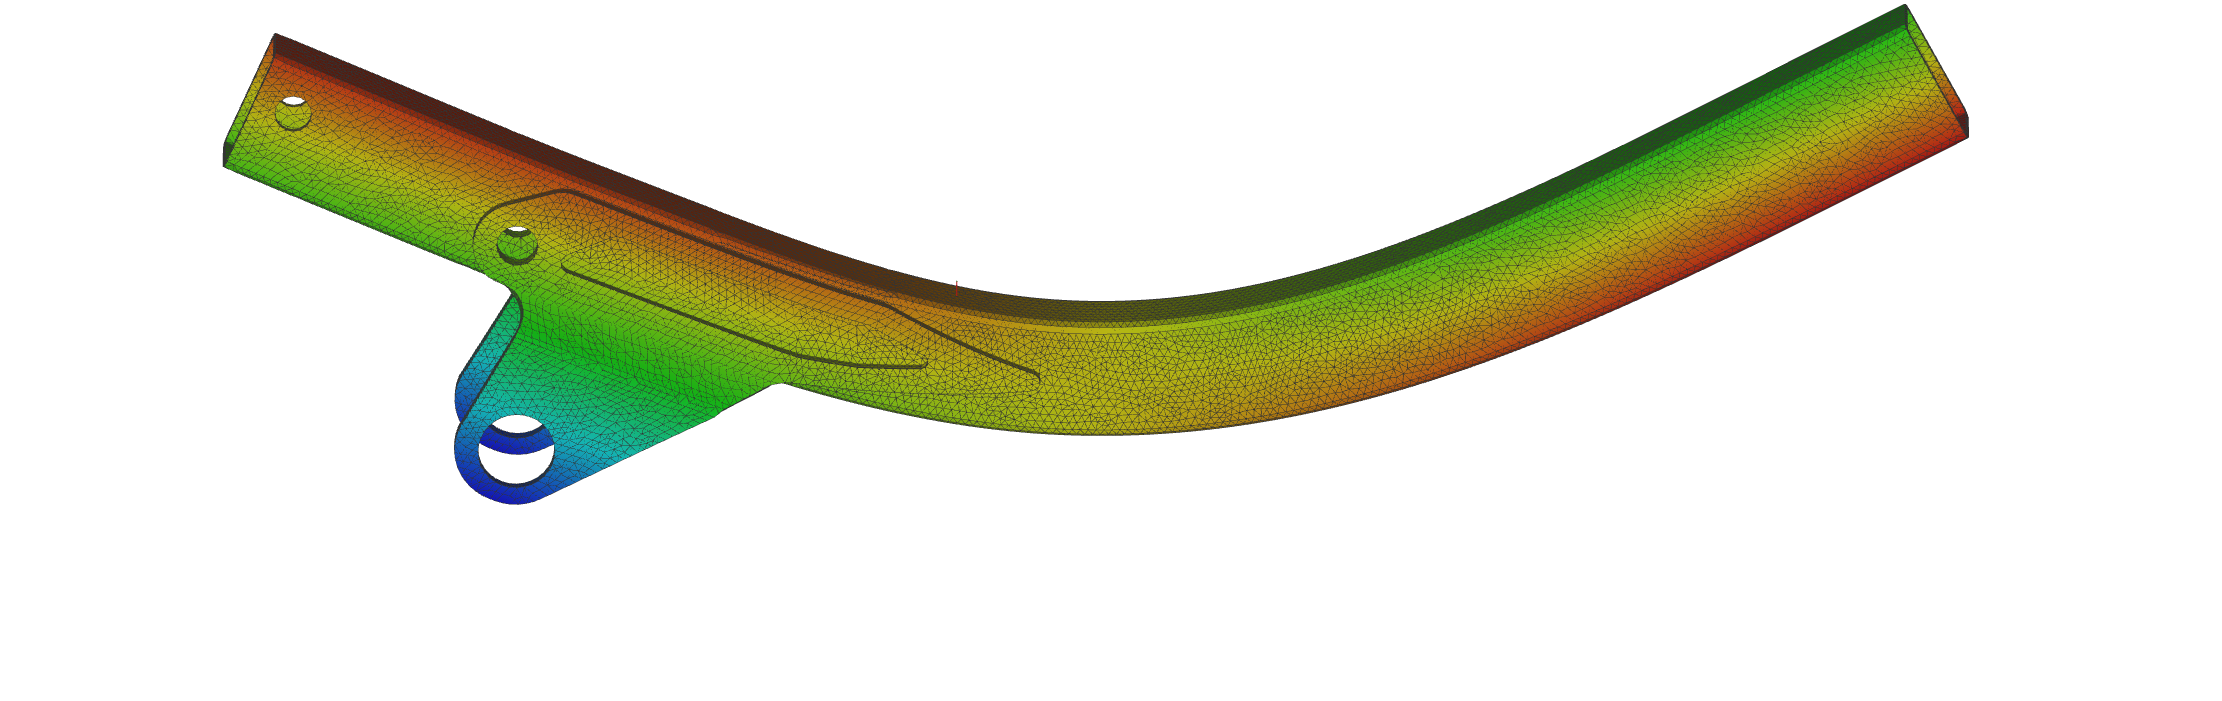
\includegraphics[width=1.82in]{TB02.png}
        \caption{194.89 Hz}
        \label{TiltSurrogate}
    \end{subfigure}
    \begin{subfigure}{0.5\textwidth} 
        \centering
        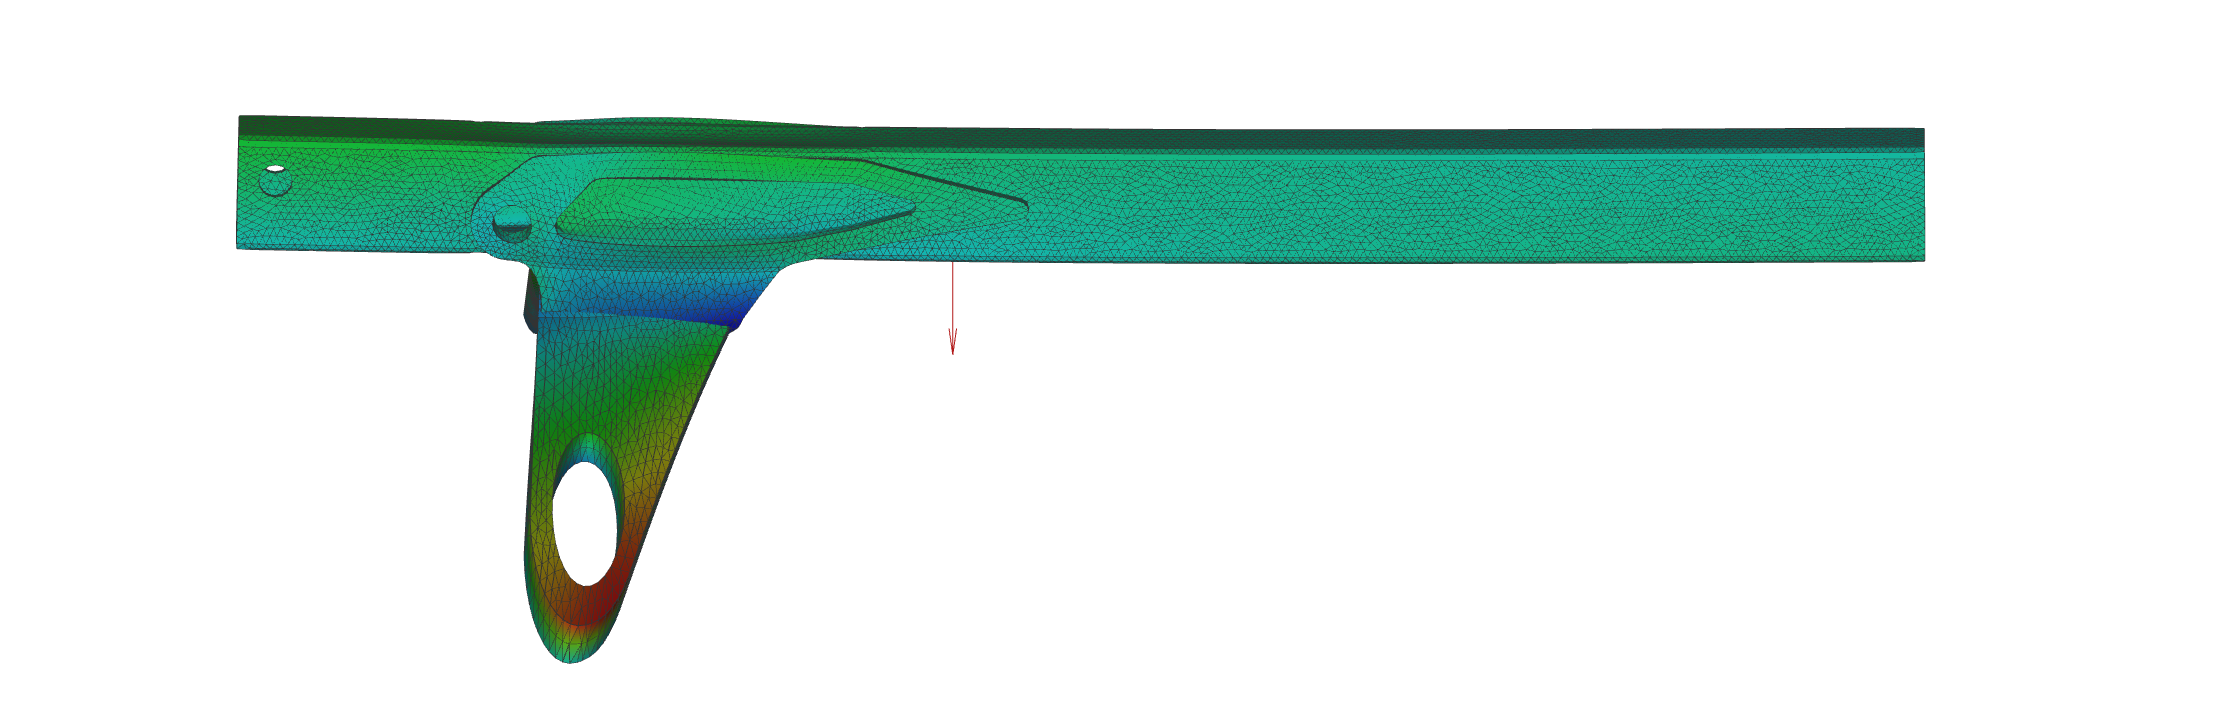
\includegraphics[width=1.82in]{TB03.png}
        \caption{276.68 Hz}
        \label{LiftSurrogate}
    \end{subfigure}%
    \begin{subfigure}{0.5\textwidth} 
        \centering
        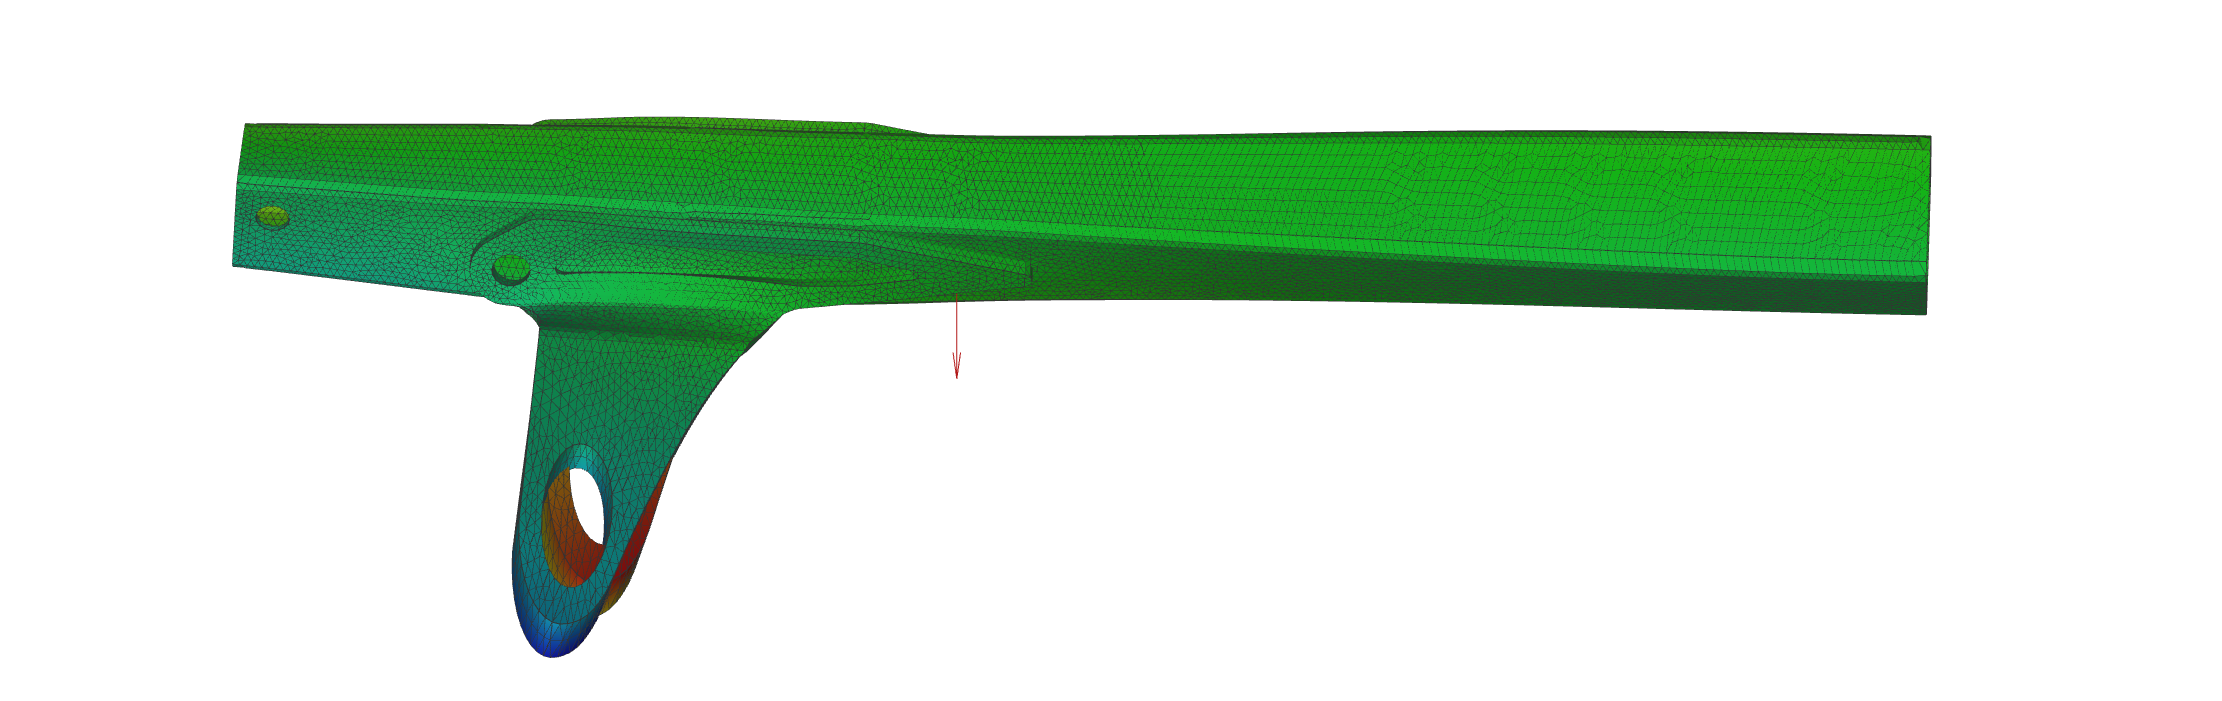
\includegraphics[width=1.82in]{TB04.png}
        \caption{332.29 Hz}
        \label{TiltSurrogate}
    \end{subfigure}
    \begin{subfigure}{0.5\textwidth} 
        \centering
        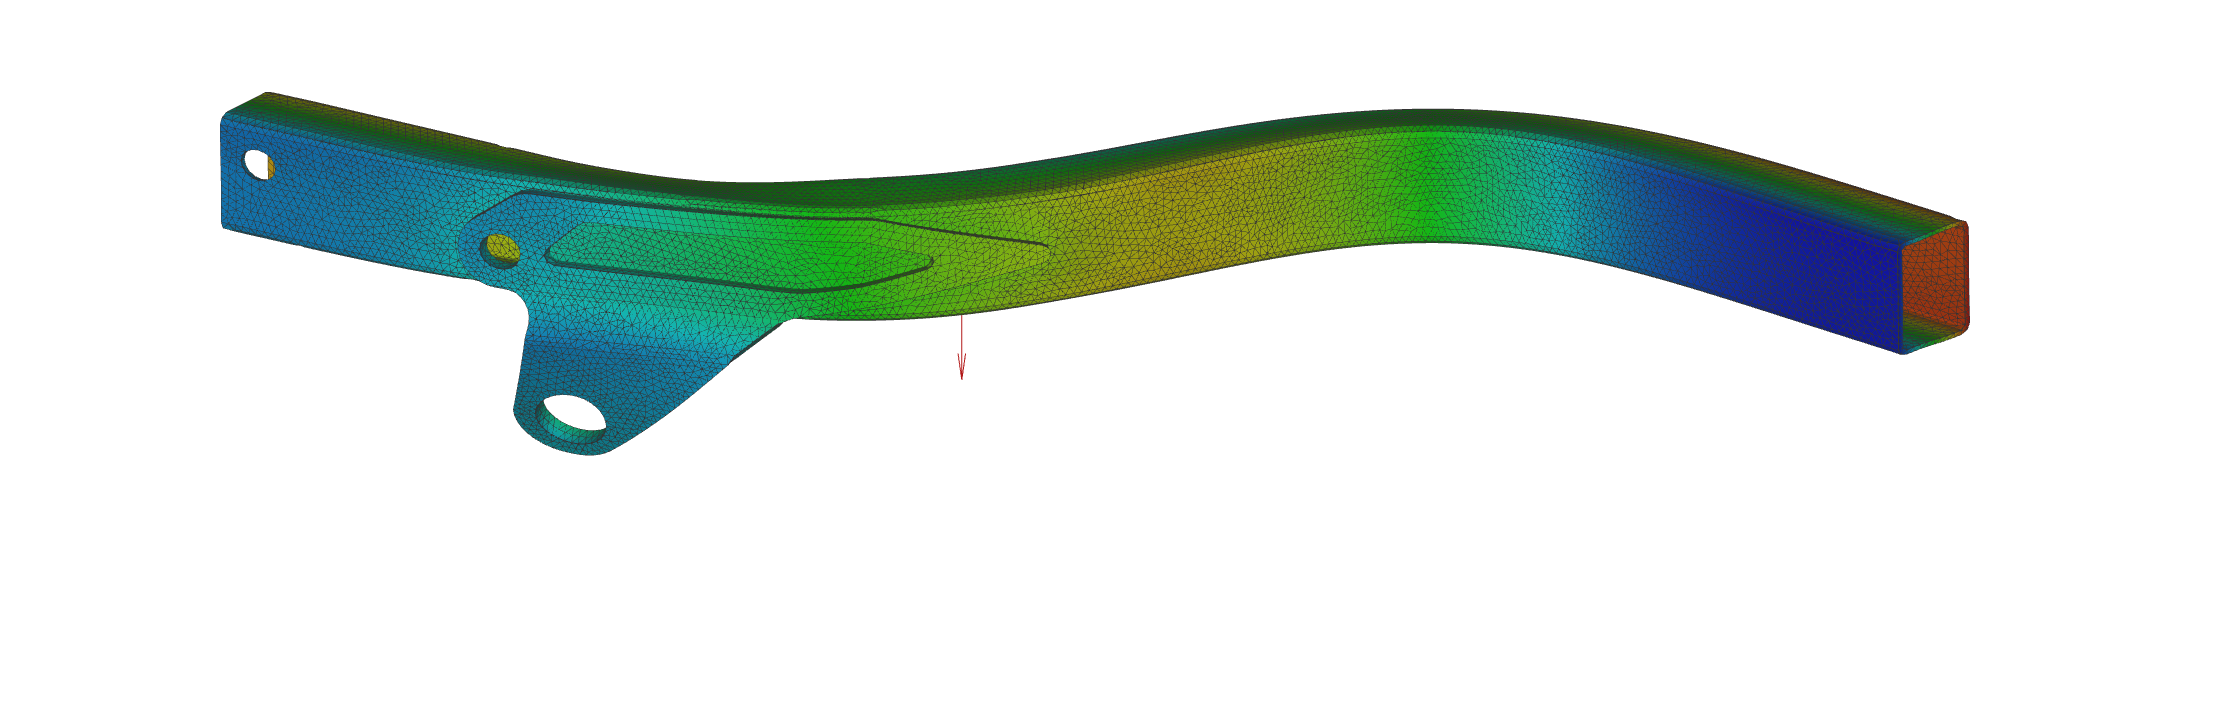
\includegraphics[width=1.82in]{TB05.png}
        \caption{406.84 Hz}
        \label{LiftSurrogate}
    \end{subfigure}%
    \begin{subfigure}{0.5\textwidth} 
        \centering
        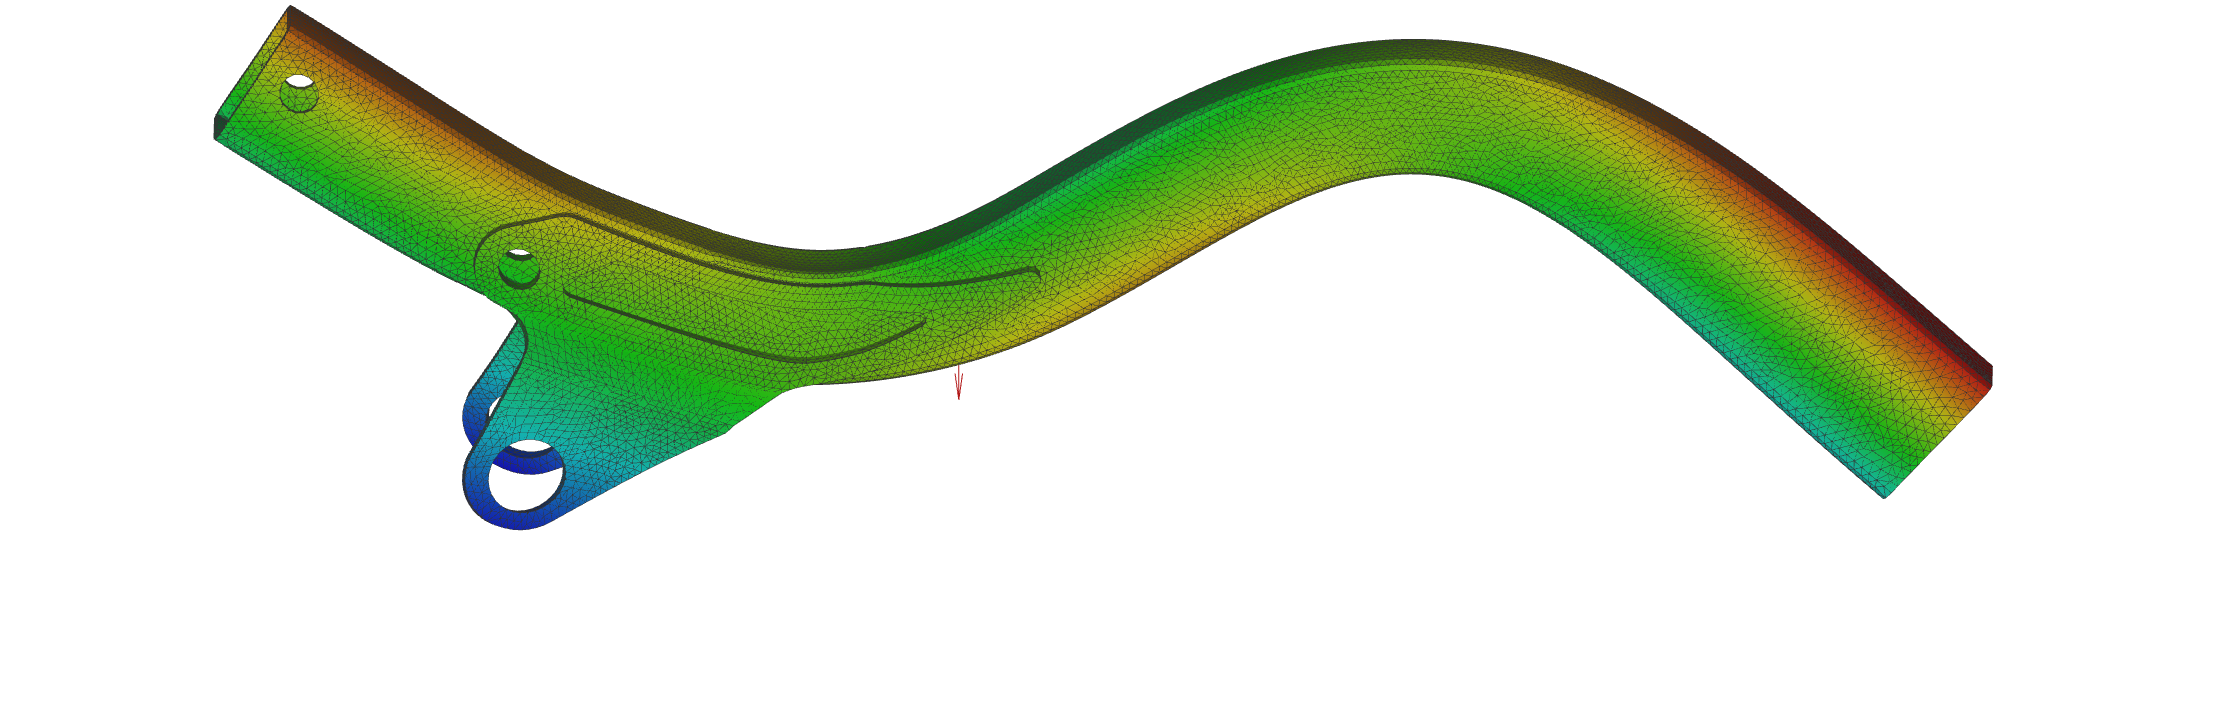
\includegraphics[width=1.82in]{TB06.png}
        \caption{521.23 Hz}
        \label{TiltSurrogate}
    \end{subfigure}
    \caption{To generate the flexible bodies, modal analysis of the lift and tilt booms was performed in ANSYS Workbench 2022 R2 using Tet4 elements. Mesh sizes were 48,319/164,092 and 31,552/102,961 (nodes/elements) for the lift boom and the tilt boom, respectively. Results were exported to Exudyn, with Craig-Bampton modal reduction applied. Modes within 100\textendash550 Hz were selected for a balance between accuracy and efficiency. The implemented modes and their frequencies are shown in (a)\textendash(f) for the lift boom and (g)\textendash(l) for the tilt boom.}
    \label{FEModel}
\end{figure}
All joints are revolute, except for a spherical joint between the two brackets. A cut joint between the brackets removes redundancy and ensures numerical stability during simulation. Rigid components serve as the default building blocks, with detailed descriptions of the rigid subsystems available in Khadim et al.~\cite{KHADIM2023105405}. However, the lift and tilt booms were modeled as flexible bodies, as they undergo the most deformation and are critical for capturing system flexibility. ANSYS Workbench 2022 R2 was used to build the finite element model, and Exudyn served as the simulation environment. The flexible body modeling process is detailed in Fig. \ref{FEModel}.
%\begin{itemize}
 %    \item \textcolor{red}{What kind of lifting loads should be included?}
%\end{itemize}
\subsection{Hydraulics}
The hydraulics in forestry crane is presented in Fig.~\ref{fig01a}. LFT has been used to model the hydraulics of forestry crane. Separate lift and tilt circuits—each consisting of a pump, tank, 4/3 directional control valve, cylinder, and piston—were connected to the respective booms. Fig.~\ref{SurrogateForestry} illustrates the system schematic. The hydraulic circuit is assumed to be ideal, with leakage neglected. A detailed description of the modeling approach and the hydraulic system’s physical parameters can be found in the study by Khadim et al~\cite{KHADIM2023105405}. The dynamic behavior of this model was analyzed and compared with the surrogate model.
% A simplified hydraulic system based on lumped fluid theory was used to actuate the forestry crane in this case study. Separate lift and tilt systems—each comprising a pump, tank, 4/3 directional control valve, cylinder, and piston—were connected to the respective booms. Figure X shows the system schematic. A detailed modeling approach for designing the mechanism can be found in the study by Khadim et al. The dynamic behavior of this model was analyzed and compared with the surrogate model.

% The hydraulic circuit is assumed ideal, with leakage neglected. FigureX shows the model parameters. The pressure values are denoted as follows: $P_p$ (pump), $P_T$ (tank), $P_1$ (lift cylinder), $P_2$ (lift piston), $P_3$ (tilt cylinder), and $P_4$ (tilt piston). The flow rates are represented by $Q_{d1}$, $Q_{d2}$, $Q_{d3}$, and $Q_{d4}$ for the lift cylinder, lift piston, tilt cylinder, and tilt piston, respectively. The lengths of the cylinder and piston sides of the lift actuator are denoted as $L_1$ and $L_2$, while $L_3$ and $L_4$ represent the corresponding values for the tilt actuator. Similarly, $V_1$, $V_2$, $V_3$, and $V_4$ denote the volumes of the cylinder and piston sides of the lift and tilt actuators, including the volume of the hoses. The input signals for the directional valves controlling the lift and tilt hydraulic systems are represented as $U_1$ and $U_2$. The hydraulic system's physical parameters are listed in Table X.

\begin{figure}[h]
    \begin{subfigure}{0.5\textwidth} 
        \centering
        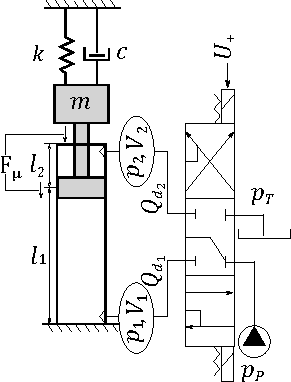
\includegraphics[width=1.82in]{Fig06a.pdf}
        \caption{Hydraulic system}
        \label{LiftSurrogate}
    \end{subfigure}%
    \hfill
    \begin{subfigure}{0.5\textwidth} 
        \centering
        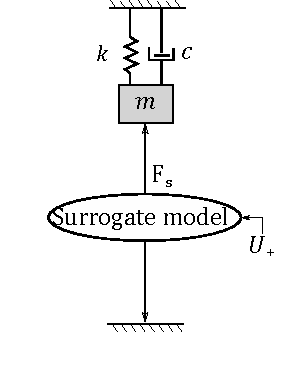
\includegraphics[width=1.82in]{Fig06b.pdf}
        \caption{Surrogate model}
        \label{TiltSurrogate}
    \end{subfigure}
    \caption{Simulation models of the hydraulics in forestry crane.}
    \label{SurrogateForestry}
\end{figure}

\subsection{Surrogate training environment}
The physics-based and surrogate models of lift and tilt cylinders of forestry crane are shown in Fig.~\ref{SurrogateForestry}. The surrogate dynamic models for the hydraulics can be described as,
\begin{equation} \label{LiftCyl_DiffEqs}
\begin{cases}
\begin{aligned}
\dot{s}_1 &= \dot{s}_1,\\[6pt]
\ddot{s}_1 &= \frac{(F_{l}+c \dot{s}_1- k_1 (s_1-x_{l_0})-{m_1}g)}{{m_1}g},\\[6pt]
\dot{s}_2 &= \dot{s}_2, \\[6pt]
\ddot{s}_2 &= \frac{(F_{t}-c_2 \dot{s}_2+ k_2 (s_2-x_{t_0}))}{m_2}.\\[6pt]
\end{aligned}
\end{cases}
\end{equation}
where $s_1$, $s_2$, $\dot{s}_1$ and $\dot{s}_2$ are positions and velocities, $k_1$ and $k_2$ are the stiffness, $c_1$ and $c_2$ are the damping of lift and tilt surrogates. The physics of both surrogates are modeled in standard Exudyn\footnote{Version 1.8, \url{https://github.com/jgerstmayr/EXUDYN}} environment.


shown in Fig.~\ref{LiftSurrogate} and Fig.~\ref{TiltSurrogate}, respectively. Exudyn\footnote{Version 1.8, \url{https://github.com/jgerstmayr/EXUDYN}} modeled the simulation models of  lift and tilt hydraulic cylinders. Simulation-driven training of universal hydraulics surrogate (UHS) is complemented by the covariance matrix adaption evolution strategy (CMA-ES)~\cite{khadim2024simulation}. An open-source Python library for CMA-ES\footnote{\url{https://pymoo.org/algorithms/soo/cmaes.html}} describes the optimization algorithm in UHS training.

The standard scipy\footnote{\url{https://scikit-learn.org/stable/modules/svm.html}} library is used to prepare data-driven surrogate with the Support vector machines (SVM). Training data in NumPy format is obtained from the Exudyn simulation models of hydraulics, presented in Fig.~\ref{LiftSurrogate} and Fig.~\ref{TiltSurrogate}. Further details about the preparation of surrogate models with both approaches can be found on the  GitHub repository. 

%\begin{itemize}   
 %   \item \textcolor{blue}{What tools should be used~(MEVEA, EXUDYN, MATLAB)?}

 %   \item \textcolor{blue}{Surrogate training in EXUDYN or MATLAB? How data is obtained? Is data generation process automated in MEVEA? }  
%\end{itemize}
\subsection{Surrogate parameters}
\begin{itemize}   
    \item \textcolor{blue}{Data-driven model (Inputs: $s$, $\dot{s}$, and $U$, Output: $F$)}

    \item \textcolor{blue}{Simulation-driven model (Optimization algorithm (CMA-ES), Objective function: Minimize the cost function $s$, $\dot{s}$ to optimize $F$)}

     \item \textcolor{blue}{Describe best NN architecture and data-drive model parameters. } 
\end{itemize}
\subsection{Implementing surrogate solutions}
\begin{itemize}   
     \item \textcolor{blue}{Implementation  in EXUDYN or MEVEA? }

    \item \textcolor{blue}{Should the results be verified with reference solution? }    
\end{itemize}
\section{Results and discussion}

This study investigated a flexible multibody dynamics system actuated by a surrogate model designed to replace a hydraulic system. As a case study, the surrogate model was used to drive a forestry crane simulated using Exudyn in a Python environment. The simulation was performed on a computer equipped with a [\textit{specify hardware configuration here}]. 

The simulation results were analyzed to assess the effects of including flexible components, replacing the hydraulic system with a surrogate model, and evaluating computational efficiency. The forestry crane was simulated for 12 seconds. Figure~\ref{Signal} shows the actuator inputs for the hydraulic model. The results for angular position, angular velocity, and structural deflections are presented in Figures~\ref{fig:comparison}, \ref{Velocity}, and \ref{StructuralDeflection}, respectively. In the result graphs, white zones indicate stationary states with no actuation input, while green zones represent extension and cyan zones indicate retraction phases of the hydraulic actuators.


\begin{figure}[ht]
    \centering
    \begin{minipage}{\textwidth}
        \centering
        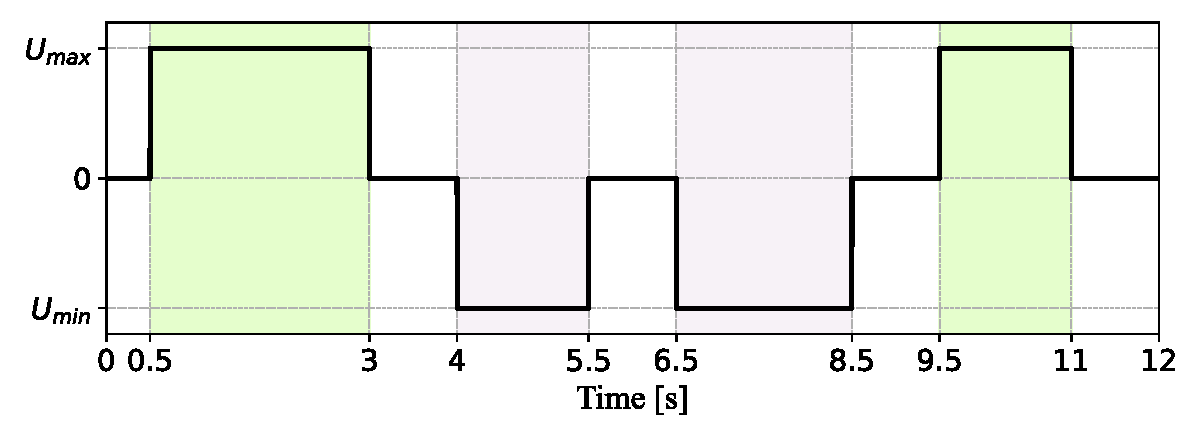
\includegraphics[width=\textwidth]{Signal-Lift.pdf}
        \subcaption{Lift hydraulic's input} \label{LiftSignal}
    \end{minipage}
    \vspace{1em}  % adds vertical space between the subfigures
    \begin{minipage}{\textwidth}
        \centering
        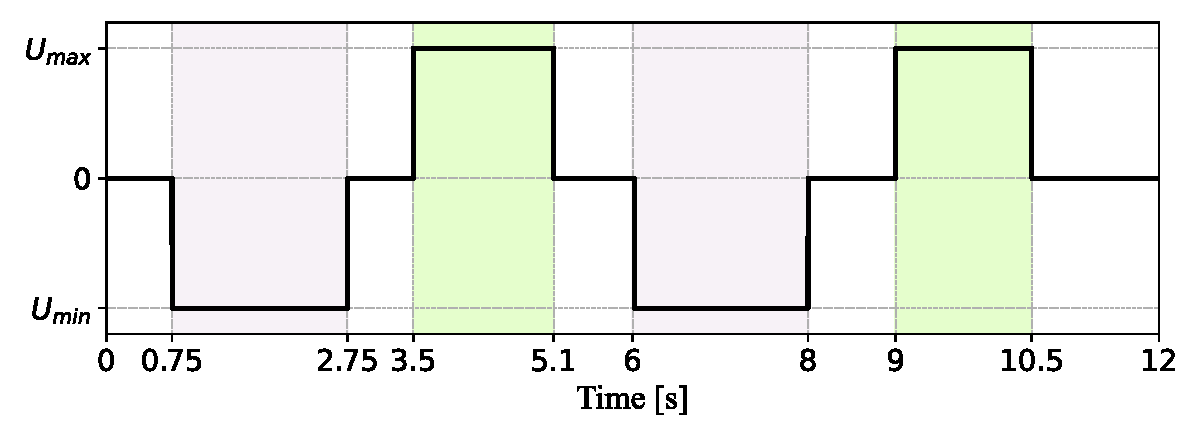
\includegraphics[width=\textwidth]{Signal-Tilt.pdf}
        \subcaption{Tilt hydraulic's input} \label{TiltSignal}
    \end{minipage}

    \caption{Hydraulics' inputs for actuating the forestry crane}
    \label{Signal}
\end{figure}

To evaluate the impact of introducing flexibility into the multibody system, the positioning of the lift and tilt booms was compared. wo angular parameters were selected: $\theta_1$, the relative angle between the lift boom and the pillar, and $\theta_2$, the relative angle between the tilt boom and the lift boom. These parameters were analyzed in both rigid and flexible configurations, with the results shown in Fig.\ref{fig:comparison}.  The values of $\theta_1$ and $\theta_2$ in the flexible configuration closely followed those in the rigid case, with only minor deviations. Additionally, small oscillations were observed in the flexible system during stationary phases (white zones), caused by rapid angular changes during deceleration. Both deviation and oscillation were more pronounced for $\theta_2$ (Fig.\ref{fig:tilt-boom}).
[\textit{Explanation to be added after discussion: What caused the deviations and oscillations in $\theta_1$ and $\theta_2$? Why were they more pronounced for $\theta_2$?}]

\begin{figure}[ht]
    \centering
    \begin{minipage}{\textwidth}
        \centering
        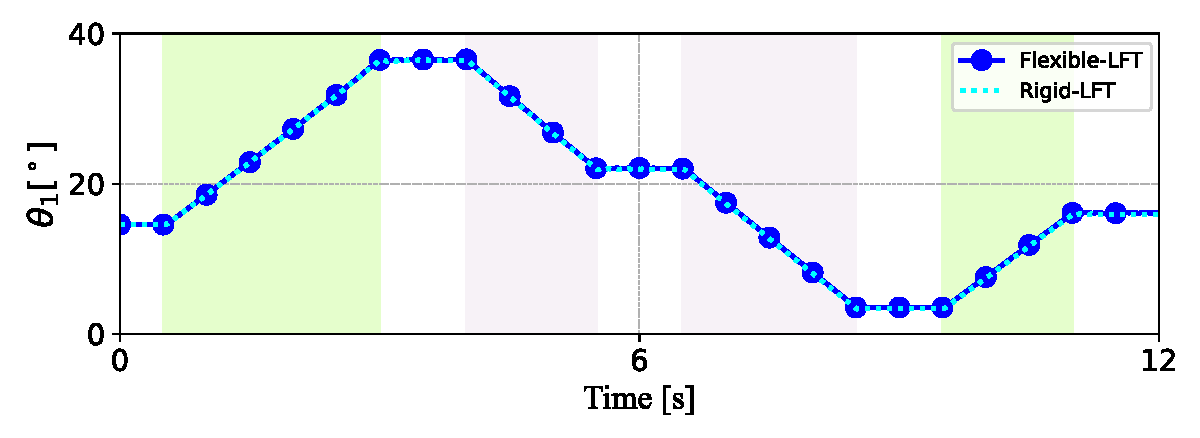
\includegraphics[width=\textwidth]{LiftAngle.pdf}
        \subcaption{Relative lift boom angle, $\theta_1$, in a working cycle of forestry crane.} \label{fig:lift-boom}
    \end{minipage}
    \vspace{1em}  % adds vertical space between the subfigures
    \begin{minipage}{\textwidth}
        \centering
        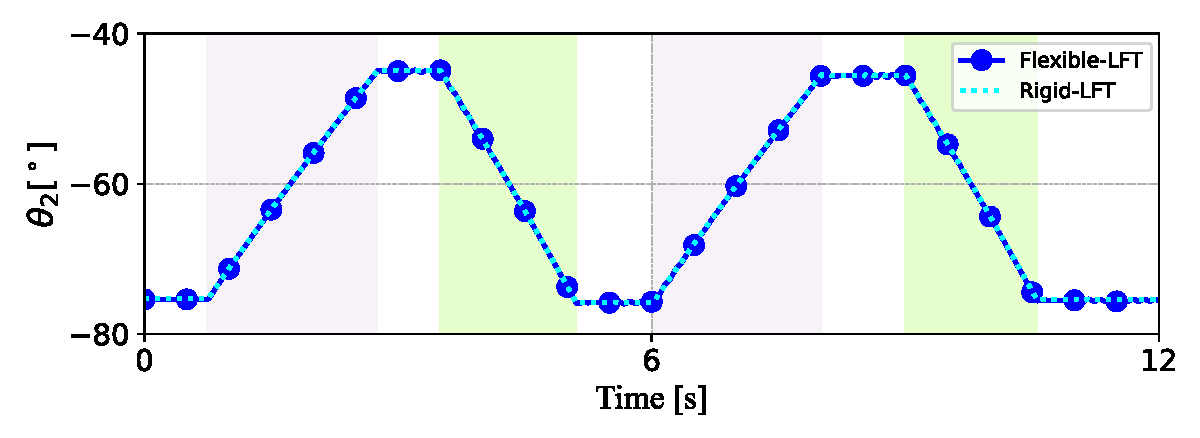
\includegraphics[width=\textwidth]{TiltAngle.pdf}
        \subcaption{Relative tilt boom angle, $\theta_2$, in a working cycle of forestry crane.} \label{fig:tilt-boom}
    \end{minipage}

    \caption{Comparing the accuracy of rigid dynamic simulation solutions with the UHS in terms of angular position.}
    \label{fig:comparison}
\end{figure}


Relative angular velocity was also analyzed to investigate the effects of flexibility on the system. The parameters $\dot{\theta}_1$ and $\dot{\theta}_2$, representing the relative angular velocities between the lift boom and pillar, and between the tilt boom and lift boom respectively, were studied in both rigid and flexible configurations (see Fig.~\ref{Velocity}). While $\dot{\theta}_1$ and $\dot{\theta}_2$ exhibited similar trends across both models, notable differences were observed. For $\dot{\theta}_1$, oscillations occurred before and after each acceleration and deceleration phase in both configurations, but these oscillations decayed faster in the rigid case. Moreover, the amplitude of the post-deceleration oscillation was significantly higher in the rigid model. In contrast, for $\dot{\theta}_2$, oscillations were present before and after each motion transition only in the flexible configuration; in the rigid configuration, they occurred only after deceleration. The amplitude of $\dot{\theta}_2$ oscillations was considerably smaller in the rigid model and also decayed more rapidly.
[\textit{Explanation to be added after discussion: What caused the oscillations? Why is the amplitude larger in the rigid lift boom but smaller in the tilt boom? What explains the faster damping in the rigid configuration?}]

\begin{figure}[ht]
    \centering
    \begin{minipage}{\textwidth}
        \centering
        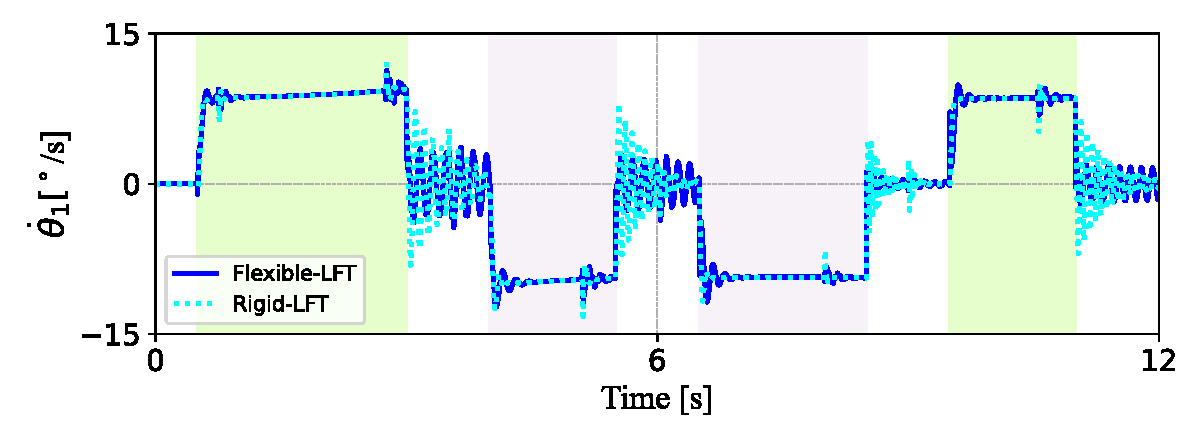
\includegraphics[width=\textwidth]{LiftVelocity.pdf}
        \subcaption{Relative lift boom angular velocity, $\dot{\theta}_1$, in a working cycle of forestry crane.} \label{LiftVelocity}
    \end{minipage}
    \vspace{1em}  % adds vertical space between the subfigures
    \begin{minipage}{\textwidth}
        \centering
        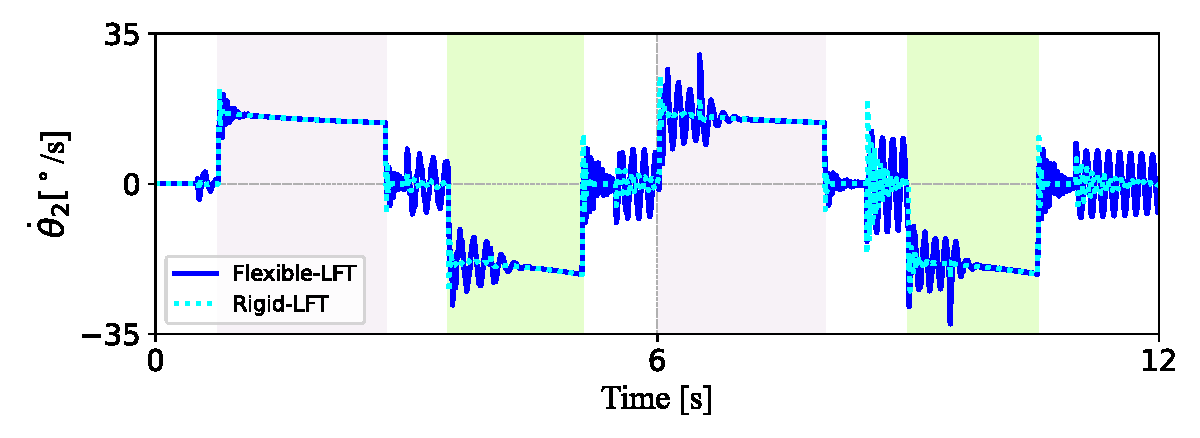
\includegraphics[width=\textwidth]{TiltVelocity.pdf}
        \subcaption{Relative tilt boom angular velocity, $\dot{\theta}_2$, in a working cycle of forestry crane.} \label{TiltVelocity}
    \end{minipage}
    \caption{Comparing the accuracy of rigid dynamic simulation solutions with the UHS in terms of angular velocity.}
    \label{Velocity}
\end{figure}

Local structural deflection was another parameter used to evaluate the flexibility of the components. The displacement of a selected node on each flexible body (see Fig.\ref{Fig:SurrogateForestry}), measured relative to its local coordinate system, was analyzed to assess structural deformation in the presence and absence of friction in the hydraulic system. Since the structure moved only within the x–y plane, the z-component of deflection was excluded.  Additionally, the deformation in the x direction (normal extension/compression) was found to be negligible. Therefore, $\delta_{y_1}$ and $\delta_{y_2}$, the local deflections along the y-axis at the tip nodes of the lift boom and tilt boom, respectively, were studied. For both $\delta_{y_1}$ and $\delta_{y_2}$, oscillations were observed during the stationary periods, indicating free vibrations triggered by transitions from dynamic motion to the stationary state. The initial value and oscillation amplitude of $\delta_{y_1}$ were higher than those of $\delta_{y_2}$ due to the initial configuration under gravity and the attachment of the tilt boom. The persistence of these oscillations further suggests a low damping ratio in the flexible model.

\begin{figure}[ht]
    \centering
    \begin{minipage}{\textwidth}
        \centering
        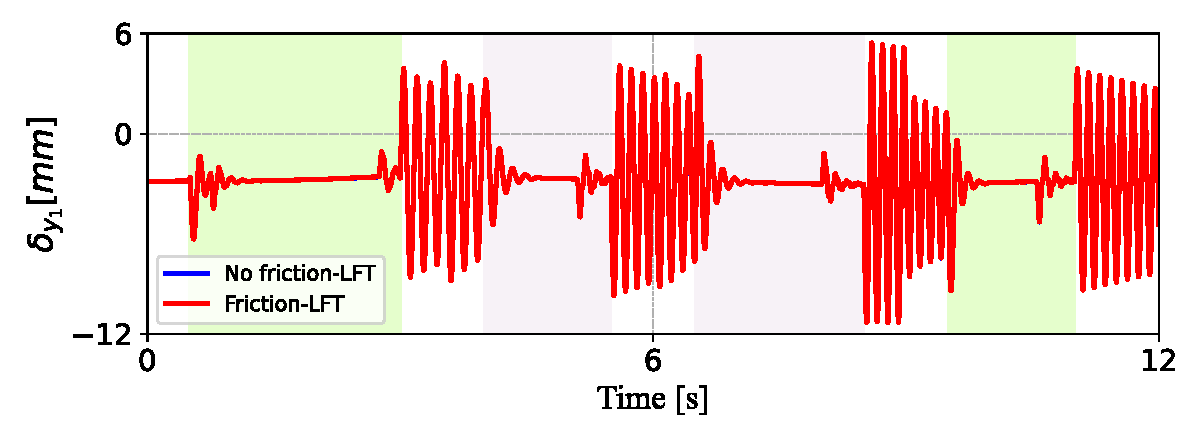
\includegraphics[width=\textwidth]{LiftDeflection.pdf}
        \subcaption{Local structural deflection at the tip of lift boom, $\delta_{y_1}$.} \label{LiftDeflection}
    \end{minipage}
    \vspace{1em}  % adds vertical space between the subfigures
    \begin{minipage}{\textwidth}
        \centering
        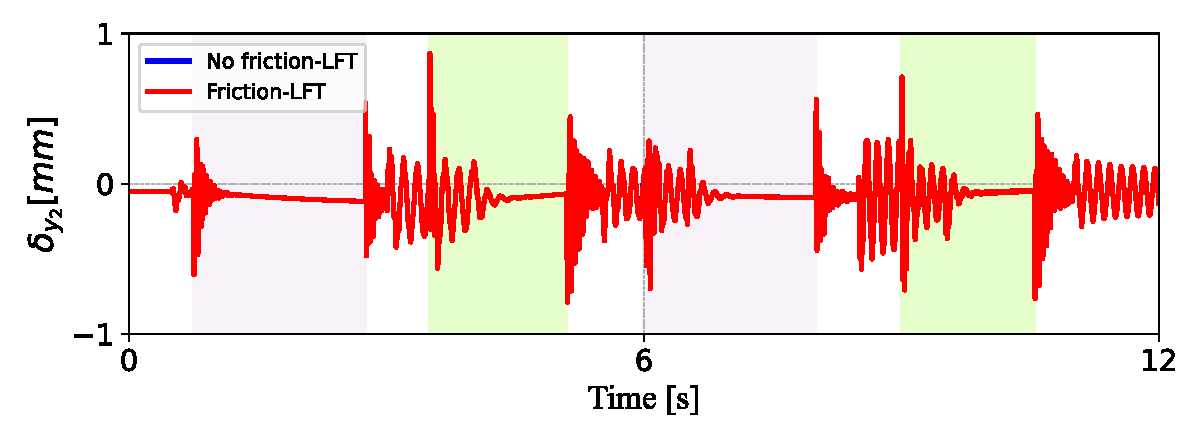
\includegraphics[width=\textwidth]{TiltDeflection.pdf}
        \subcaption{Local structural deflection at the tip of tilt boom, $\delta_{y_2}$} \label{TiltDeflection}
    \end{minipage}
    \caption{Structural deflections in lift and tilt booms during a working cycle in the presence and absence of the friction.}
    \label{StructuralDeflection}
\end{figure}

\subsection{Training performance}
\begin{itemize}   
    \item \textcolor{blue}{Comparing training performance of data-driven and simulation-driven models?}

    \item \textcolor{blue}{How much data and time are needed for the surrogate models?}
     
\end{itemize}
\subsection{Predictions in the working cycle of crane}





% \begin{figure}[ht]
%     \centering
%     \begin{minipage}{\textwidth}
%         \centering
%         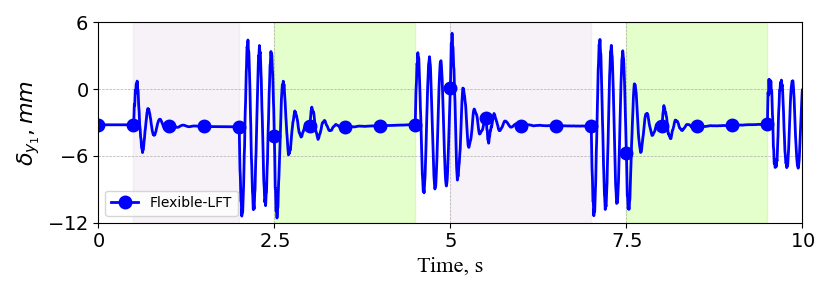
\includegraphics[width=\textwidth]{LiftDeflection.png}
%         \subcaption{Local structural deflection at the tip of lift boom, $\delta_{y_1}$.} \label{Def1}
%     \end{minipage}
%     \vspace{1em}  % adds vertical space between the subfigures
%     \begin{minipage}{\textwidth}
%         \centering
%         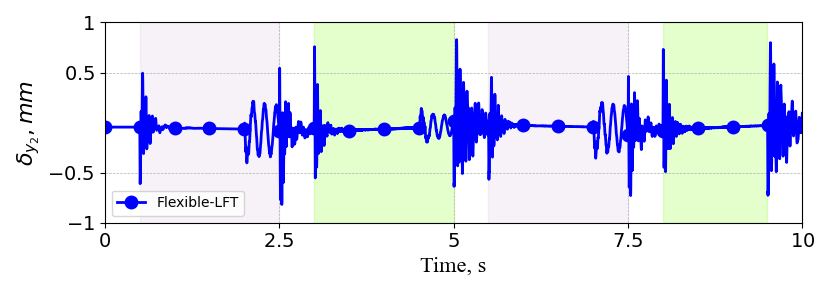
\includegraphics[width=\textwidth]{TiltDeflection.png}
%         \subcaption{Local structural deflection at the tip of tilt boom, $\delta_{y_2}$} \label{Def2}
%     \end{minipage}
%     \caption{Structural deflections in lift and tilt booms during a working cycle.}
%     \label{fig:Defs}
% \end{figure}



%\begin{figure}
%\begin{subfigure}{.5\textwidth}
 % \centering
  %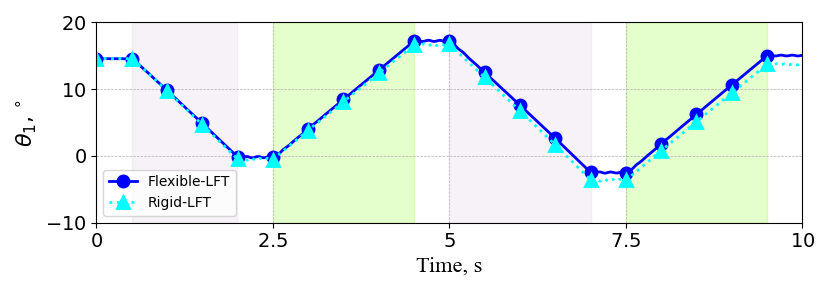
\includegraphics[width=\linewidth]{angle1.png}
  %\caption{Lift boom angle~$z_1$.}
  %\label{Angle_fb}
%\end{subfigure}%
%\hfill
%\begin{subfigure}{.5\textwidth}
 % \centering
  %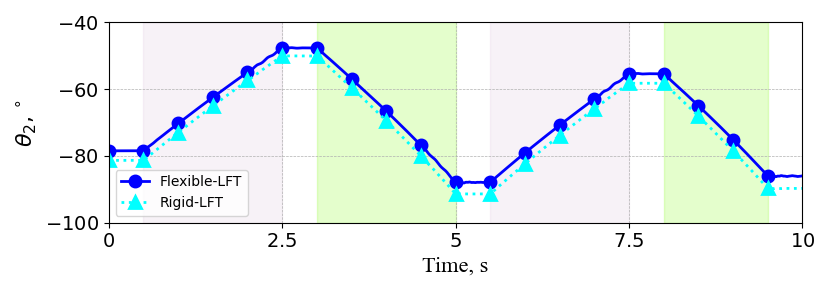
\includegraphics[width=\linewidth]{angle2.png}
  %\caption{Tilt boom angle~$z_2$}
  %\label{AngularVelocity_fb}
%\end{subfigure}
%\begin{subfigure}{.5\textwidth}
 % \centering
  %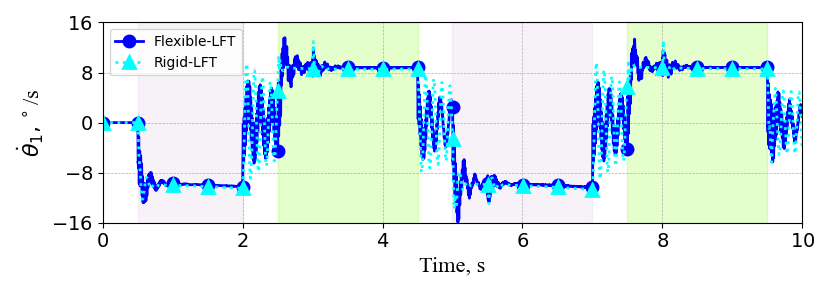
\includegraphics[width=\linewidth]{angularVelocity1.png}
  %\caption{Lift boom angular velocity~$\dot{z}_1$.}
  %\label{Angle_Liftpt}
%\end{subfigure}%
%\hfill
%\begin{subfigure}{.5\textwidth}
 % \centering
 % 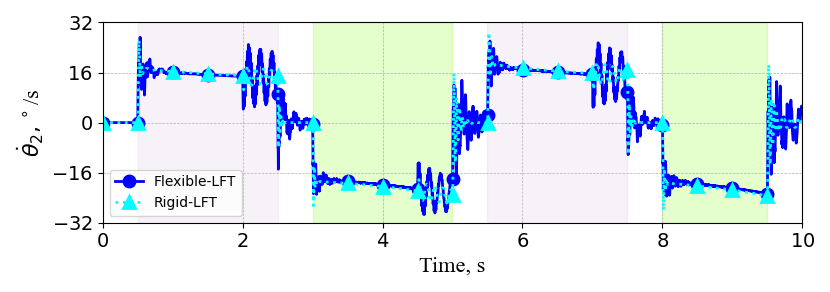
\includegraphics[width=\linewidth]{angularVelocity2.png}
  %\caption{Tilt boom angular velocity $\dot{z}_2$}
  %\label{AngularVelocity_Liftpt}
%\end{subfigure} 
%\caption{Comparing the accuracy of rigid dynamic simulation solutions with the UHS.}
%\label{AccuracyFlexiblePATU_1mode}
%\end{figure}

\begin{itemize}   
    \item \textcolor{blue}{Should the control signal be fixed?}

    \item \textcolor{blue}{What should be compared? Actuator movements? Tip-displacements? Deflections or strains? Stresses?}

    \item \textcolor{blue}{Comparing rigid and flexible with LFT, NN and simulation-driven  ?}

    \item \textcolor{blue}{How many combinations?}

       \item \textcolor{blue}{Computational efficiency?}
       
          \item \textcolor{blue}{Accuracy?}
     
\end{itemize}

\section{Conclusion}

In the manuscript, a novel enhanced surrogate hydraulic model that coupled a flexible multibody system and modal reduction techniques to further improve the computational efficiency. The methodology is demonstrated in the forestry crane application. As a summary, the proposed workflow \\
- Proposes a working working work flow that is having improved computational efficiency and yet high accuracy in a forestry crane application \\
- Computational efficiency yy \%?\\
- Accuracy xx \% \\

For the scienficic community, this proposed workflow shows that the computational efficiency can be improved without sacrificing the accuracy significantly. However, it should be noted that the algorithms could be further optimized for a specific usage thereby creating opportunities for further research to achieve even better results as shown in this study.

For further studies extension to assess the loads and optimization of the flexible structure and mode selection process. 
\begin{itemize}
    \item \textcolor{red}{What were the objectives and goal?}
    
    \item \textcolor{red}{Were the objectives achieved?}

    \item \textcolor{red}{Implications?}

       \item \textcolor{red}{Benefits of approach in the scientific and business communities?}
\end{itemize}

%\begin{acknowledgements}
%If you'd like to thank anyone, place your comments here
%and remove the percent signs.
%\end{acknowledgements}


% Authors must disclose all relationships or interests that 
% could have direct or potential influence or impart bias on 
% the work: 
%
% \section*{Conflict of interest}
%
% The authors declare that they have no conflict of interest.


% BibTeX users please use one of
%\bibliographystyle{spbasic}      % basic style, author-year citations
%\bibliographystyle{spmpsci}      % mathematics and physical sciences
%\bibliographystyle{spphys}       % APS-like style for physics
%\bibliography{}   % name your BibTeX data base

% Non-BibTeX users please use
% \begin{thebibliography}{}
% % %
% % % and use \bibitem to create references. Consult the Instructions
% % % for authors for reference list style.
% %
% \bibitem{RefJ}
% % Format for Journal Reference
% Author, Article title, Journal, Volume, page numbers (year)
% % Format for books
% \bibitem{RefB}
% Author, Book title, page numbers. Publisher, place (year)
% % etc
% \end{thebibliography}
\bibliography{Biblography}
\end{document}
% end of file template.tex

